\documentclass[12pt]{article}
\usepackage[margin=1in]{geometry} 
\usepackage{tabularx}
\geometry{letterpaper}   


\usepackage{amssymb,amsfonts,amsmath,bbm,mathrsfs,stmaryrd, mathtools}
\usepackage{xcolor}
\usepackage{url}
\usepackage{dsfont}
\usepackage{enumerate}
\usepackage{enumitem}
\usepackage{tikz-cd}
\usetikzlibrary{cd}

%\usepackage{parskip}

\usepackage[colorlinks,
             linkcolor=black!75!red,
             citecolor=blue,
             pdftitle={},
             pdfauthor={},
             pdfproducer={pdfLaTeX},
             pdfpagemode=None,
             bookmarksopen=true
             bookmarksnumbered=true]{hyperref}

\usepackage{tikz}
\usetikzlibrary{cd,arrows,calc,decorations.pathreplacing,decorations.markings,intersections,shapes.geometric,through,fit,shapes.symbols,positioning,decorations.pathmorphing}

\usepackage{braket}

\renewcommand{\theequation}{\thesection.\arabic{equation}}

%%%%%%%%%%%%%%%%%%%%%%%%%%%%%%%%
%%% Theorems and references %%%
%%%%%%%%%%%%%%%%%%%%%%%%%%%%%%%%
\usepackage[amsmath,thmmarks,hyperref]{ntheorem}
\usepackage{cleveref}

\creflabelformat{enumi}{#2(#1)#3}

\crefname{section}{Section}{Sections}
\crefformat{section}{#2Section~#1#3} 
\Crefformat{section}{#2Section~#1#3} 

\crefname{subsection}{\S}{\S\S}
\crefformat{subsection}{#2\S#1#3} 
\Crefformat{subsection}{#2\S#1#3} 

\theoremstyle{plain}

\newtheorem{lemma}{Lemma}[section]
\newtheorem{proposition}[lemma]{Proposition}
\newtheorem{corollary}[lemma]{Corollary}
\newtheorem{theorem}[lemma]{Theorem}
\newtheorem{conjecture}[lemma]{Conjecture}
\newtheorem{question}[lemma]{Question}
\newtheorem{assumption}[lemma]{Assumption}


\theoremstyle{nonumberplain}
\newtheorem{theoremN}{Theorem}
\newtheorem{propositionN}{Proposition}
\newtheorem{corollaryN}{Corollary}


\theoremstyle{plain}
\theorembodyfont{\upshape}
\theoremsymbol{\ensuremath{\blacklozenge}}

\newtheorem{definition}[lemma]{Definition}
\newtheorem{example}[lemma]{Example}
\newtheorem{remark}[lemma]{Remark}
\newtheorem{convention}[lemma]{Convention}
\newtheorem{exercise}[lemma]{Exercise}

\crefname{definition}{definition}{definitions}
\crefformat{definition}{#2definition~#1#3} 
\Crefformat{definition}{#2Definition~#1#3} 

\crefname{ex}{example}{examples}
\crefformat{example}{#2example~#1#3} 
\Crefformat{example}{#2Example~#1#3} 

\crefname{remark}{remark}{remarks}
\crefformat{remark}{#2remark~#1#3} 
\Crefformat{remark}{#2Remark~#1#3} 

\crefname{convention}{convention}{conventions}
\crefformat{convention}{#2convention~#1#3} 
\Crefformat{convention}{#2Convention~#1#3} 

\crefname{exercise}{exercise}{exercises}
\crefformat{exercise}{#2exercise~#1#3} 
\Crefformat{exercise}{#2Exercise~#1#3} 



\crefname{lemma}{lemma}{lemmas}
\crefformat{lemma}{#2lemma~#1#3} 
\Crefformat{lemma}{#2Lemma~#1#3} 

\crefname{proposition}{proposition}{propositions}
\crefformat{proposition}{#2proposition~#1#3} 
\Crefformat{proposition}{#2Proposition~#1#3} 

\crefname{corollary}{corollary}{corollaries}
\crefformat{corollary}{#2corollary~#1#3} 
\Crefformat{corollary}{#2Corollary~#1#3} 

\crefname{theorem}{theorem}{theorems}
\crefformat{theorem}{#2theorem~#1#3} 
\Crefformat{theorem}{#2Theorem~#1#3} 

\crefname{assumption}{assumption}{Assumptions}
\crefformat{assumption}{#2assumption~#1#3} 
\Crefformat{assumption}{#2Assumption~#1#3} 

\crefname{equation}{}{}
\crefformat{equation}{(#2#1#3)} 
\Crefformat{equation}{(#2#1#3)}

\theoremstyle{nonumberplain}
\theoremsymbol{\ensuremath{\blacksquare}}

\newtheorem{proof}{Proof.}
\newtheorem{solution}{Solution.}
\newcommand\pf[1]{\newtheorem{#1}{Proof of \Cref{#1}.}}

%%%%%%%%%%%%%%%%%%%%%%%%%%%%%%%%%%%%%%%%%%%%%%%%%%%%%%%%%%%%%
%%%%%%%%%%%%%%%%%%% simple math operators %%%%%%%%%%%%%%%%%%%
%%%%%%%%%%%%%%%%%%%%%%%%%%%%%%%%%%%%%%%%%%%%%%%%%%%%%%%%%%%%%
\DeclareMathOperator{\id}{id}
\DeclareMathOperator{\End}{\mathrm{End}}
\DeclareMathOperator{\pr}{\mathrm{Prob}}
\DeclareMathOperator{\orb}{\mathrm{Orb}}


\DeclareMathOperator{\cact}{\cat{CAct}}
\DeclareMathOperator{\wact}{\cat{WAct}}

%%%%%%%%%%%%%%%%%%%%%%%%%%%%%%%%%%%%%%%%%%%%%%%%%%%%%%%%%%
%%% align* numbering %%%
%%%%%%%%%%%%%%%%%%%%%%%%%%%%%%%%%%%%%%%%%%%%%%%%%%%%%%%%%%

\newcommand\numberthis{\addtocounter{equation}{1}\tag{\theequation}}



%%%%%%%%%%%%%%%%%%%%%%%%%%%%%%%%%%%%%%%%%%%%%%%%%%%%%%%%%%%%
%%%%%%%%%%%%%%%%%%%%%%%%%%%%%%%%%%%%%%%%%%%%%%%%%%%%%%%%%%%%
%%%%%%%%%%%%%%%%%%%%%%%%%%%%%%%%%%%%%%%%%%%%%%%%%%%%%%%%%%%%
%% user macros
%%%%%%%%%%%%%%%%%%%%%%%%%%%%%%%%%%%%%%%%%%%%%%%%%%%%%%%%%%%%
%%%%%%%%%%%%%%%%%%%%%%%%%%%%%%%%%%%%%%%%%%%%%%%%%%%%%%%%%%%%
%%%%%%%%%%%%%%%%%%%%%%%%%%%%%%%%%%%%%%%%%%%%%%%%%%%%%%%%%%%%

% below are many macros
% be careful...

%%%%%%%%%%%%%%%%%%%%%%%%%%%%%%%%%%%%%%%%%%%%%%%%%%%%%%%%%%
%%% misc (should not need to touch) %%%
%%%%%%%%%%%%%%%%%%%%%%%%%%%%%%%%%%%%%%%%%%%%%%%%%%%%%%%%%%

\newcommand\ol{\overline}
\newcommand\wt{\widetilde}

%
\newcommand{\define}[1]{{\em #1}}
\newcommand\1{{\bf 1}}
\newcommand{\cat}[1]{\textsc{#1}}
\newcommand\mathify[2]{\newcommand{#1}{\cat{#2}}}
\newcommand\spr[1]{\cite[\href{https://stacks.math.columbia.edu/tag/#1}{Tag {#1}}]{stacks-project}}
\newcommand{\qedhere}{\mbox{}\hfill\ensuremath{\blacksquare}}


\renewcommand{\square}{\mathrel{\Box}}
\newcommand\Section[1]{\section{#1}\setcounter{lemma}{0}}

%%%%%%%%%%%%%%%%%%%%%%%%%%%%%%%%
%% math fonts
%%%%%%%%%%%%%%%%%%%%%%%%%%%%%%%%


% math blackboard font

\newcommand\bb[1]{{\mathbb #1}} 

\newcommand\bA{{\mathbb A}}
\newcommand\bB{{\mathbb B}}
\newcommand\bC{{\mathbb C}}
\newcommand\bD{{\mathbb D}}
\newcommand\bE{{\mathbb E}}
\newcommand\bF{{\mathbb F}}
\newcommand\bG{{\mathbb G}}
\newcommand\bH{{\mathbb H}}
\newcommand\bI{{\mathbb I}}
\newcommand\bJ{{\mathbb J}}
\newcommand\bK{{\mathbb K}}
\newcommand\bL{{\mathbb L}}
\newcommand\bM{{\mathbb M}}
\newcommand\bN{{\mathbb N}}
\newcommand\bO{{\mathbb O}}
\newcommand\bP{{\mathbb P}}
\newcommand\bQ{{\mathbb Q}}
\newcommand\bR{{\mathbb R}}
\newcommand\bS{{\mathbb S}}
\newcommand\bT{{\mathbb T}}
\newcommand\bU{{\mathbb U}}
\newcommand\bV{{\mathbb V}}
\newcommand\bW{{\mathbb W}}
\newcommand\bX{{\mathbb X}}
\newcommand\bY{{\mathbb Y}}
\newcommand\bZ{{\mathbb Z}}

% math script font

\newcommand\cA{{\mathcal A}}
\newcommand\cB{{\mathcal B}}
\newcommand\cC{{\mathcal C}}
\newcommand\cD{{\mathcal D}}
\newcommand\cE{{\mathcal E}}
\newcommand\cF{{\mathcal F}}
\newcommand\cG{{\mathcal G}}
\newcommand\cH{{\mathcal H}}
\newcommand\cI{{\mathcal I}}
\newcommand\cJ{{\mathcal J}}
\newcommand\cK{{\mathcal K}}
\newcommand\cL{{\mathcal L}}
\newcommand\cM{{\mathcal M}}
\newcommand\cN{{\mathcal N}}
\newcommand\cO{{\mathcal O}}
\newcommand\cP{{\mathcal P}}
\newcommand\cQ{{\mathcal Q}}
\newcommand\cR{{\mathcal R}}
\newcommand\cS{{\mathcal S}}
\newcommand\cT{{\mathcal T}}
\newcommand\cU{{\mathcal U}}
\newcommand\cV{{\mathcal V}}
\newcommand\cW{{\mathcal W}}
\newcommand\cX{{\mathcal X}}
\newcommand\cY{{\mathcal Y}}
\newcommand\cZ{{\mathcal Z}}

% math frak font

\newcommand\fA{{\mathfrak A}}
\newcommand\fB{{\mathfrak B}}
\newcommand\fC{{\mathfrak C}}
\newcommand\fD{{\mathfrak D}}
\newcommand\fE{{\mathfrak E}}
\newcommand\fF{{\mathfrak F}}
\newcommand\fG{{\mathfrak G}}
\newcommand\fH{{\mathfrak H}}
\newcommand\fI{{\mathfrak I}}
\newcommand\fJ{{\mathfrak J}}
\newcommand\fK{{\mathfrak K}}
\newcommand\fL{{\mathfrak L}}
\newcommand\fM{{\mathfrak M}}
\newcommand\fN{{\mathfrak N}}
\newcommand\fO{{\mathfrak O}}
\newcommand\fP{{\mathfrak P}}
\newcommand\fQ{{\mathfrak Q}}
\newcommand\fR{{\mathfrak R}}
\newcommand\fS{{\mathfrak S}}
\newcommand\fT{{\mathfrak T}}
\newcommand\fU{{\mathfrak U}}
\newcommand\fV{{\mathfrak V}}
\newcommand\fW{{\mathfrak W}}
\newcommand\fX{{\mathfrak X}}
\newcommand\fY{{\mathfrak Y}}
\newcommand\fZ{{\mathfrak Z}}

\newcommand\fa{{\mathfrak a}}
\newcommand\fb{{\mathfrak b}}
\newcommand\fc{{\mathfrak c}}
\newcommand\fd{{\mathfrak d}}
\newcommand\fe{{\mathfrak e}}
\newcommand\ff{{\mathfrak f}}
\newcommand\fg{{\mathfrak g}}
\newcommand\fh{{\mathfrak h}}
%\newcommand\fi{{\mathfrak i}}
\newcommand\fj{{\mathfrak j}}
\newcommand\fk{{\mathfrak k}}
\newcommand\fl{{\mathfrak l}}
\newcommand\fm{{\mathfrak m}}
\newcommand\fn{{\mathfrak n}}
\newcommand\fo{{\mathfrak o}}
\newcommand\fp{{\mathfrak p}}
\newcommand\fq{{\mathfrak q}}
\newcommand\fr{{\mathfrak r}}
\newcommand\fs{{\mathfrak s}}
\newcommand\ft{{\mathfrak t}}
\newcommand\fu{{\mathfrak u}}
\newcommand\fv{{\mathfrak v}}
\newcommand\fw{{\mathfrak w}}
\newcommand\fx{{\mathfrak x}}
\newcommand\fy{{\mathfrak y}}
\newcommand\fz{{\mathfrak z}}


\newcommand\fgl{\mathfrak{gl}}
\newcommand\fsl{\mathfrak{sl}}
\newcommand\fsp{\mathfrak{sp}}


%%%%%%%%%%%%%%%%%%%%%%%%%%%%%%%%%%%%%%%%%%%%%%%%%%%%%%%%%%
%%% QIT useful commands %%%
%%%%%%%%%%%%%%%%%%%%%%%%%%%%%%%%%%%%%%%%%%%%%%%%%%%%%%%%%%

\newcommand{\bmat}[1]{\begin{bmatrix*} #1 \end{bmatrix*}} % matrices
\newcommand{\setovecs}[1]{\lb \ket{v_1}, \ldots, \ket{v_{#1}}\rb} % set of vectors
\newcommand{\listovecs}[2]{\ket{{#1}_1}, \ldots, \ket{{#1}_{#2}}} % set list of NAMED vectors
\newcommand{\Tr}{\text{Tr}} % trace v1
\newcommand{\tr}{\text{tr}} % trace v2
\newcommand{\proj}[2]{\ket{#1}\bra{#2}}

%%%%%%%%%%%%%%%%%%%%%%%%%%%%%%%%%%%%%%%%%%%%%%%%%%%%%%%%%%
%%% standard mitch commands %%%
%%%%%%%%%%%%%%%%%%%%%%%%%%%%%%%%%%%%%%%%%%%%%%%%%%%%%%%%%%

%% Standard Sets
\newcommand{\Q}{\mathbb{Q}} % rationals
\newcommand{\R}{\mathbb{R}} % reals
\newcommand{\Z}{\mathbb{Z}} % integers
\newcommand{\C}{\mathbb{C}} % complex numbers
\newcommand{\N}{\mathbb{N}} % natural numbers
\newcommand{\F}{\mathbb{F}} % arbitrary field
\newcommand{\T}{\mathbb{T}} % Unit circle
\newcommand{\D}{\mathbb{D}} % Open unit disc

%% Arrows
\newcommand{\ra}{\rightarrow}
\newcommand{\Ra}{\Rightarrow}
\newcommand{\La}{\Leftarrow}

%% Greek
\newcommand{\al}{\alpha}
\newcommand{\ep}{\varepsilon} % epsilon
\newcommand{\es}{\varnothing} % empty set


%% Brackets
\newcommand{\<}{\left\langle} 
\renewcommand{\>}{\right\rangle}
\newcommand{\lp}{\left(}
\newcommand{\rp}{\right)}
\newcommand{\lv}{\left\lvert}
\newcommand{\rv}{\right\rvert}
\newcommand{\lb}{\left\{}
\newcommand{\rb}{\right\}}
\newcommand{\lan}{\left\langle}
\newcommand{\ran}{\right\rangle}

%% Algebra
\newcommand{\isom}{\cong} %Isomorphic
\newcommand{\nsub}{\trianglelefteq} %Normal Subgroup
\newcommand{\semi}{\rtimes} %Semi-Direct Product
\newcommand{\Aut}{\text{Aut}} % automorphism group
\newcommand{\op}{{\text{op}}} % opposite algebra

%% Linear Algebra
\newcommand{\norm}[1]{\left\lVert#1\right\rVert} % norm
\newcommand{\inp}[2]{\left\langle#1\mid #2\right\rangle} % inner product
\newcommand{\spn}[1]{\text{Span}\lp #1\rp} % span
\newcommand{\cspn}[1]{\overline{\text{Span}}\lp #1\rp} % closed span

%% Analysis
\newcommand{\abs}[1]{\left\lvert #1 \right\rvert} % absolute value
\newcommand{\supp}[1]{\text{supp}\lp #1\rp} % support
\newcommand{\co}{\text{co}} % convex hull
\newcommand{\cl}[1]{\overline{#1}} % closure
\DeclareMathOperator*{\esssup}{ess\,sup} % essential supremum

%% Complex 
\newcommand{\Res}[2]{\text{Res}\lp #1, #2\rp} %Residue of a FUNCTION at a POINT
\newcommand{\Ind}{\text{Ind}} % index
\newcommand{\re}[1]{\text{Re}(#1)}  % real part
\newcommand{\im}[1]{\text{Im}(#1)} % complex part

\newcommand{\sinx}[1]{\sin\left(#1\right)}
\newcommand{\cosx}[1]{\cos\left(#1\right)}

%% QIT
\newcommand{\setofkets}[1]{\lb \ket{#1_1}, \ket{#1_2}, \ldots, \ket{#1_n}\rb} % Set of ket vectors


%%!!!!!!!!!!!!!!!!!!!!!!!!!!!!!!!!!!!!!!!!!!!!!!!!!!!!!!!!!!!!!!!!!!!!!!!!!!!!
%%!!!!!!!!!!!!!!!!!!!!!!!!!!!!!!!!!!!!!!!!!!!!!!!!!!!!!!!!!!!!!!!!!!!!!!!!!!!!
%%!!!!!!!!!!!!!!!!!!!!!!!!!!!!!!!!!!!!!!!!!!!!!!!!!!!!!!!!!!!!!!!!!!!!!!!!!!!!
% start of document
%%!!!!!!!!!!!!!!!!!!!!!!!!!!!!!!!!!!!!!!!!!!!!!!!!!!!!!!!!!!!!!!!!!!!!!!!!!!!!
%%!!!!!!!!!!!!!!!!!!!!!!!!!!!!!!!!!!!!!!!!!!!!!!!!!!!!!!!!!!!!!!!!!!!!!!!!!!!!
%%!!!!!!!!!!!!!!!!!!!!!!!!!!!!!!!!!!!!!!!!!!!!!!!!!!!!!!!!!!!!!!!!!!!!!!!!!!!!

%%%%%%%%%%%%%%%%%%%%%%%%%%%%%%%%%%%%%%%
%%%%%%%%%%%%%%%%%%%%%%%%%%%%%%%%%%%%%%%
%%%%%
% Title and Document Info
%%%%%
%%%%%%%%%%%%%%%%%%%%%%%%%%%%%%%%%%%%%%%
%%%%%%%%%%%%%%%%%%%%%%%%%%%%%%%%%%%%%%%

\title{MA 399 Intro to Quantum Information Theory}
\author{Hayden Roszell}
\date{\today}

\begin{document}
\maketitle
\begin{abstract}
Modern trends seem to conclude that the future of information processing will be increasingly completed using quantum computers. As opposed to their classical counterparts, quantum computers operate according to quantum mechanics. Quantum information theory discusses the possibilities and limitations of information representation and communication over quantum channels. This paper gives an overview of the inner workings of the math used by quantum information theory, and provides examples of the benefits over classical information theory.
\end{abstract}

\tableofcontents

\section{Intro to Vector Spaces}

Let's jump right in. This section is an abbreviation of the introduction to linear algebra session.

A vector space is a group of objects (vectors) which may be added together and multiplied by compatible scalars from $\R$ or $\C$. In this class, we primarily care about vector spaces $\C^n$ over $\C$ and $\R^n$ over $\R$. Recall that $\C$ is the scalar field of complex numbers $a+bi$, where multiplication is defined by the rule $i^2=-1$, and is equipped with:
\begin{enumerate}[label=(\alph*)]
    \item a complex conjugation operation -- $\ol{a+bi}=(a+bi)^*=a-bi$ and
    \item a size function called the \textbf{modulus} -- $\abs{a+bi}=\sqrt{a^2+b^2}.$
\end{enumerate}
Note that the modulus is similar to magnitude. \\
To work with complex numbers, it's useful to have an understanding of the basic operations.
\begin{enumerate}[label=(\alph*)]
	\item To add/subtract complex numbers, add/subtract the corresponding real/imaginary parts. For 		example -- $(a+bi)+(c+di)=(a+c)+(b+d)i$
	\item To multiply/divide complex numbers, multiply both parts of the complex number by the real 		number. For example -- $(a+bi)*(c+di)=ac+adi+bcj-bd=(ac-bd)+(ad+bc)i$. This form will be useful 		for the duration of the class.
\end{enumerate}

%%%%%%%%%%%%%%%%%%%%%%%%%%%%%%%%%%%%%%%%%%%%%%%%%%%%%%%%%%
%%% Representing Vectors in Complex Spaces %%%
%%%%%%%%%%%%%%%%%%%%%%%%%%%%%%%%%%%%%%%%%%%%%%%%%%%%%%%%%%

\subsection{Representing Vectors in Complex Spaces}
As mentioned, this class primarily works in complex number spaces. For this reason, having useful tools for representing vectors in these abstract spaces is useful. Vectors are represented in \textbf{bra-ket} notation, where \textit{bra} represents a \textit{row} vector, and \textit{ket} represents a \textit{column} vector.

\begin{definition}\label{def:ket}
If $\ket{v}\in\C^n$ is a \textit{ket} vector which consists of $n$ complex numbers,
\begin{equation}
\ket{v}=\bmat{v_1 \\ v_2 \\ ... \\ v_n} \textrm{for } v_1, v_2, ..., v_n \in \C
\end{equation}
\end{definition}

\begin{definition}\label{def:bra}
If $\bra{v}\in\C^n$ is a \textit{bra} vector which consists of $n$ complex numbers,
\begin{equation}
\bra{v}=\bmat{v_1 & v_2 & ... & v_n} \textrm{for } v_1, v_2, ..., v_n \in \C
\end{equation}
\end{definition}
Note that the the integer $n$ in definitions \ref{def:ket} and \ref{def:bra} is called the \textbf{dimension} of the vector space $\C^n$.

\begin{example}
$\C^2$ is a 2-dimensional vector space over $\C$.
\begin{center}
$\alpha\bmat{1 \\ 0} + \beta\bmat{0 \\ 1}$ \\
$\bmat{\alpha \\ 0}+\bmat{0 \\ \beta}=\bmat{\alpha \\ \beta}$
Note: $\bmat{\alpha \\ \beta}$ 'fills up' $\C^2$; IE it represents all values contained within $\C^2$
\end{center}
\end{example}

%%%%%%%%%%%%%%%%%%%%%%%%%%%%%%%%%%%%%%%%%%%%%%%%%%%%%%%%%%
%%% Linear Combinations %%%
%%%%%%%%%%%%%%%%%%%%%%%%%%%%%%%%%%%%%%%%%%%%%%%%%%%%%%%%%%

\subsection{Linear Combinations}
A linear combination is a useful tool for this class which is the 'combination' or multiplication of each term in a set by constants, and then adding the result. The interesting property of linear combinations is that the result is still contained within the initial set.

\begin{definition}\label{def:li}
A linear combination of $\lbrace\ket{v_1}, ..., \ket{v_n}\rbrace\subset\C^n$ is a single vector in the form $\lambda_1\ket{v_1} + \lambda_2\ket{v_2} + ... + \lambda_n\ket{v_n}$ for some $\lambda_1, \lambda_2, ... , \lambda_k\in\C^n$.
\end{definition}

\begin{remark}
If $\ket{w}$ is a linear combination of $\lbrace\ket{v_1}, ..., \ket{v_n}\rbrace\subset\C^n$, we can say that it belongs to the \textbf{span} of the set of $\lbrace\ket{v_1}, ..., \ket{v_n}\rbrace\subset\C^n$.
\end{remark}

\begin{example}
Create a linear combination of $\ket{v_1}=\bmat{i \\ 2}, \ket{v_2}=\bmat{-1 \\ i+1}$
\begin{center}
(\textit{foil}) \\
$(3+2i)\bmat{i \\ 2} + (2+i)\bmat{-1 \\ i+1}$ \\
(\textit{add}) \\
$=\bmat{3i-2 \\ 6+4i} + \bmat{-2-i \\ 3i+1}$ \\
$=\bmat{2i-4 \\ 7i+7}=\ket{w}$ \textit{spans} $\lbrace\ket{v_1}, \ket{v_2}\rbrace$
\end{center}
\end{example}

%%%%%%%%%%%%%%%%%%%%%%%%%%%%%%%%%%%%%%%%%%%%%%%%%%%%%%%%%%
%%% Linear Independence %%%
%%%%%%%%%%%%%%%%%%%%%%%%%%%%%%%%%%%%%%%%%%%%%%%%%%%%%%%%%%

\subsection{Linear Independence}
Another important concept is that of a set being \textit{linearly independent}. Being linearly independent essentially means that every piece of 'information' given by a set of vectors adds some sort of new information/perspective on the problem.

\begin{remark}
Two vectors are \textbf{linearly independent} as long as they are not \textit{parallel}.
\end{remark}

A good way of looking at this is that a system that is not linearly independent has more than one element that is some offset of the same constant. These elements are not giving new perspective, because they give the same information.

\begin{definition}
A set of vectors $\setovecs{v}$ is linearly independent if no vector is a linear combination of any other vectors. Algebraically, if $\lambda_1\ket{v_1} + \lambda_2\ket{v_2} + ... + \lambda_n\ket{v_k}=\ket{0}, \text{ then } \lambda_1=\lambda_2=\lambda_k=0$
\end{definition}

The only way that the zero vector ($\ket{0}$) can be possible is if the complex constants ($\lambda$) are all the same, \textit{and} zero.

\begin{theorem}
If a set of $k$ vectors in $\C^n$ is linearly independent, then $k \leq n$. Equivalently, if you have a set of $k$ vectors in $\C^n$ such that $k>n$, then the set is linearly dependent.
\end{theorem}

This theorem is important because it establishes the notion that a set can't contain more vectors than the space allows for. Said differently, the dimension of $M$ is the number of vectors contained within that can be linearly independent.

%%%%%%%%%%%%%%%%%%%%%%%%%%%%%%%%%%%%%%%%%%%%%%%%%%%%%%%%%%
%%% Basis %%%
%%%%%%%%%%%%%%%%%%%%%%%%%%%%%%%%%%%%%%%%%%%%%%%%%%%%%%%%%%

\subsection{Basis}
\begin{theorem}
A \textbf{basis} of a subspace $M\subseteq\C^n$ is a set of vectors such that
\begin{enumerate}
	\item $S$ is linearly independent
	\item $\spn{S}$ $=M$ $\Longrightarrow$ \textit{S Spans M}
\end{enumerate}
\end{theorem}
It follows that the standard basis of $\C^n$ is $\bmat{1 \\ 0 \\ 0 \\ ... \\ 0},\bmat{0 \\ 1 \\ 0 \\ ... \\ 0},\bmat{0 \\ 0 \\ 1 \\ ... \\ 0},\bmat{0 \\ 0 \\ 0 \\ ... \\ 1}$

%%%%%%%%%%%%%%%%%%%%%%%%%%%%%%%%%%%%%%%%%%%%%%%%%%%%%%%%%%
%%% Inner Products %%%
%%%%%%%%%%%%%%%%%%%%%%%%%%%%%%%%%%%%%%%%%%%%%%%%%%%%%%%%%%

\subsection{Inner Products}

Recall that $\ket{v}$ is a column vector and $\bra{v}$ is a row vector. Before talking about inner products, we must define operations that help the inner product process.
\begin{remark}
$(\C^n)^*$ is the \textit{dual space} of $\C^n$.
\end{remark}
The dual space is the space of all row vectors. This is useful for the next definition, which is critical in completing inner products.
\begin{definition}
We equip $\C^n$ with an "involution" (\textit{conjugate transpose}) operation:
\begin{center}
$\dagger:\C^n\longrightarrow(\C^n)^*$ given by $\bmat{x_1 \\ ... \\ x_n}=\bmat{x_1^* & ... & x_n^*}$ given a $\ket{v}\in\C^n$, $\bra{v}=\ket{v}^\dagger$
\end{center}
\end{definition}
A quick example of this operation is helpful to explain the significance of these definitions.
\begin{example}
Given $\ket{v}=\bmat{7 \\ 8i \\ \pi + 3i \\ 0}\in\C^4$, find $\ket{v}^\dagger$\\
Take the complex conjugate of each entry \\
$\bra{v}=\bmat{7 & -8i & \pi-3i & 0}$
\end{example}
Now, we can talk about inner products. Of primary importance for this section, the inner product can determine if two vectors are orthogonal, and operates the same as a dot product on $\R^n$.
\begin{definition}
Given $\ket{v}, \ket{w}\in\C^n$, the \textbf{inner product} of $\ket{v}$ and $\ket{w}$ is $\langle w|v \rangle=\bra{w}^\dagger\cdot\ket{v}$
\end{definition}
\begin{remark}
The inner product on $\R^n$ is the usual dot product.
\end{remark}
The following is a simple example showing the inner product on simple vectors in $\R^3$.
\begin{example}
Given $\ket{v}=\bmat{1 \\ 1\\ 3}, \ket{w}=\bmat{5 \\ -2 \\ 1}\in\R^3$, find $\langle w|v \rangle$ \\
\indent Perform a complex conjugate on $\ket{w}$ (In $\R^3$, this is the same as flipping $nx1$ to $1xn$) \\
\indent $\langle w|v \rangle=\bmat{5 & -2 & 1}\cdot\bmat{1 \\ 1 \\ 3}=(5*1)+(-2*1)+(1*3)=6$
\end{example}
Now, the following example shows the inner product on two simple vectors in $\C^2$.
\begin{example}\label{ex:cpcmp}
Given $\ket{v}=\bmat{i \\ 1}, \ket{w}=\bmat{i \\ -1}\in\C^2$, find $\inp{w}{v}$
\begin{center}
$\inp{w}{v}=\bmat{-i & -1}\cdot\bmat{i \\ 1}=1+(-1*1)=0$
\end{center}
\end{example}
Recall from calculus III that the dot product of two vectors can give us insight on orthogonality. In the case of example \ref{ex:cpcmp}, the inner product of $\langle w|v \rangle$ was zero. This tells us that the two vectors are orthogonal.
\begin{definition}
The \textbf{norm} (similar to magnitude) of $\ket{v}\in\C^n$ is $\norm{\ket{v}}:=\sqrt{\inp{v}{v}}$ 
\end{definition}
\begin{example}
$\ket{v}=\bmat{1 \\ 1}\in\R^2\longrightarrow||\ket{v}||=\sqrt{1^2+1^2}=\sqrt{2}$
\end{example}
\begin{remark}
\begin{itemize}
	\item $\ket{v}\in\C^n$ with $||\ket{v}||=1$ is called a unit vector
	\item Unit vectors in $\C^n$ represent a \textit{quantum state}
	\item An important property of a norm is the \textit{triangle inequality} $\longrightarrow\norm{\ket{v}+\ket{w}}\leq\norm{\ket{v}}+\norm{\ket{w}}$
\end{itemize}
\end{remark}
\begin{definition}
A set of non-zero vectors $S=\setofkets{v}\leq\C^n$ is called an orthogonal set if $\inp{v_i}{w_j}=0$ if $i\neq j$
\end{definition}
\begin{theorem}
If $S=\setofkets{v}$ is an orthogonal set of non-zero vectors in $\C^n$, then $S$ is linearly independent.
\end{theorem}
\begin{proof}
Let $c_1, ..., c_k\in\C$ such that $c_1\ket{v_1}+...+c_k\ket{v_k}=\ket{0}$. \\
\textit{Goal: show that $c_1=c_2=c_k=0\longrightarrow$ linearly independent using $S$ is orthogonal} \\
Additionally, let \\ 
\indent $j\in{1,...,k}$.\\
Then, \\ 
\indent $\bra{v_j}(c_1\ket{v_1}+...+c_k)=\inp{v_j}{0}$ \\
\indent $\longrightarrow c_1\inp{v_j}{v_1}+...+c_k\inp{v_j}{v_k}$ \\
\indent $c_j\inp{v_j}{v_j}=$ (\textit{$v_j$ is the only component allowed to have magnitude}) \\
Thus, $c_j=0$ since $\ket{v_j}\neq\ket{0}$ \\
Note: Since $j$ was arbitrary, $c_1 = c_2 = ... = c_k = 0$. Hence, $S$ is linearly independent.
\end{proof}

\begin{remark}
$S$ is an orthonormal basis if:
\begin{itemize}
	\item $S$ is an orthonormal set if $n$ unit vectors
	\item $\spn{S}=\C^n$
\end{itemize}
\end{remark}

%%%%%%%%%%%%%%%%%%%%%%%%%%%%%%%%%%%%%%%%%%%%%%%%%%%%%%%%%%
%%% Projections %%%
%%%%%%%%%%%%%%%%%%%%%%%%%%%%%%%%%%%%%%%%%%%%%%%%%%%%%%%%%%

\subsection{Projections}

\begin{definition}
Define $\ket{f_i}\bra{f_i}$ to be the \textbf{projection} operator onto $\spn{\ket{f_i}}$
\end{definition}

\begin{theorem}
Let $\beta=\setofkets{f}$ be an orthonormal basis for $\C^n$. Then, any $\ket{x}=c_1\ket{f_1}+...+c_n\ket{f_n}=\inp{f_1}{x}\ket{f_1}+...+\inp{f_n}{x}\ket{f_n}$.
\end{theorem}
It follows that $\sum_{j=1}^{n} \ket{f_j}\bra{f_j}=\bmat{1 &  &  \\  & \ddots &  \\  &  &  1}$

\begin{example}
Let $\ket{f_1}=\frac{-2}{\sqrt{2}}\bmat{1 \\ 1},\ket{x}=\bmat{-2 \\ 1}$. \\
$\ket{x_|}=\inp{f_1}{x}\ket{f_1}$ \\
$P_1(\ket{x})=\ket{f_1}\inp{f_1}{x}$
\end{example}
In the above example, $\ket{x_|}$ is the projection of $x$ onto $f_1$ in the direction of $f_1$.
Note that the projection operation is similar to \textit{comp} from calculus III. Now, let's look at some properties of the projection operator.
\begin{proposition}
Let $\beta=\setofkets{f}$ be an orthonormal basis for $\C^n$. Then, $\lbrace P_1, P_2, P_n\rbrace$ is a set of $n\times n$ matrices such that
\begin{enumerate}
\item $P_i(\ket{v})\in\spn{\ket{f_i}}$
\item $\ket{v}-P_i(\ket{v})$ is orthogonal to $\ket{f_i}$
\item $P_i^2=P_i*P_i=P_i$
\item $P_iP_j=0$ when $i\neq\j$, and $P_i^\dagger=P_i$
\item $\sum_{i=1}^{n} P_i=I_n$ IE the sum of $P$'s gives us the identity matrix.
\end{enumerate}
\end{proposition}

Projection operators make it easy for us to find $c_1, c_2, c_n$ for $\ket{x}=c_1\ket{f_1}+...+c_k\ket{f_k}$ when $\setofkets{f}$ is an orthonormal set. Side note, in quantum land, $P_i$'s are how we measure the probability that $\ket{x}$ is actually in $\ket{f_i}$.

%%%%%%%%%%%%%%%%%%%%%%%%%%%%%%%%%%%%%%%%%%%%%%%%%%%%%%%%%%
%%% Gram-Schmidt %%%
%%%%%%%%%%%%%%%%%%%%%%%%%%%%%%%%%%%%%%%%%%%%%%%%%%%%%%%%%%

\subsection{Gram-Schmidt}

Let $\beta=\setofkets{b}$ be a basis for $\C^n$
\begin{itemize}
\item Linearly independent
\item $\spn{\beta}=\C^n$ (IE no redundancy)
\end{itemize}
Goal: Turn $\beta$ into an orthonormal basis, $\setofkets{f}$
\begin{enumerate}
\item First, make an orthogonal basis. \\
$\ket{f_{i+1}}:=\ket{b_{i+1}}-(\sum_{j=1}{i} \frac{\inp{f_j}{b_{i+1}}}{\inp{f_j}{f_j}}\ket{f_j})$
\item Then, make an orthonormal basis by normalizing the resultant ($\ket{f}$) vectors. \\
For each $\ket{f}$, $\ket{f}=\frac{1}{\norm{\ket{f}}}\ket{f}$
\end{enumerate}

%%%%%%%%%%%%%%%%%%%%%%%%%%%%%%%%%%%%%%%%%%%%%%%%%%%%%%%%%%
%%% Exercise 1 %%%
%%%%%%%%%%%%%%%%%%%%%%%%%%%%%%%%%%%%%%%%%%%%%%%%%%%%%%%%%%

\subsection{Exercise 1}
\textbf{Consider $S={\ket{v_1}, \ket{v_2}, \ket{v_3}}$ where $\ket{v_1}=\bmat{1 \\ -1}, \ket{v_2}=\bmat{i \\ 1}, \ket{v_3}=\bmat{0 \\ i}$}
\begin{enumerate}[label=(\alph*)]
	\item \textbf{Give a linear combination of the vectors in $S$.} \\
	\begin{center}
	$\alpha\bmat{1 \\ -1} + \beta\bmat{i \\ 1} + \gamma\bmat{0 \\ i}=\ket{w}$ \\
	\end{center}
	Note that the next problem asks to determine if a vector is in span($S$). To 'kill two birds with 		one stone', try to find a linear combination that 			satisfies the question. To do this, assign 			values for $\alpha$, $\beta$, and $\gamma$. Note that $1+i=i+i$ (the top row), and $-1+1=0$. This
	allows us to set $\alpha$ and $\beta$ to $1$ and operate on $\gamma$.
	\begin{center}
	$i(x+yi)=200-i$ \\
	$xi-y$ $\Longrightarrow$ $x=-1$ $\Longrightarrow$ $\gamma=-1i-200$
	\end{center}
	Now plug in values.
	$1*\bmat{1 \\ -1} + 1*\bmat{i \\ 1} + (-200-1i)*\bmat{0 \\ i}=\ket{w}$
	\item \textbf{Determine if $\bmat{1+i \\ 200-i}$ in Span($S$)} \\
	Start with where we left off in the last part.
	\begin{center}
	$1*\bmat{1 \\ -1} + 1*\bmat{i \\ 1} + (-200-1i)*\bmat{0 \\ i}=\bmat{1+i \\ 200-i}$
	\end{center}
	$\bmat{1+i \\ 200-i}$ \textit{is} in Span($S$) because there existed values $\alpha$, $\beta$, and 	$\gamma$ such that $\ket{w}$ of $S$ is a possible outcome of $S$.
	\item \textbf{Describe Span($S$) "geometrically"} \\
	Span($S$) can be thought of as every possible vector $(\alpha\bmat{1 \\ -1} + \beta\bmat{i \\ 1} + 	\gamma\bmat{0 \\ i})$ contained within $\C^2$
	
\end{enumerate}

%%%%%%%%%%%%%%%%%%%%%%%%%%%%%%%%%%%%%%%%%%%%%%%%%%%%%%%%%%
%%% Exercise 2 %%%
%%%%%%%%%%%%%%%%%%%%%%%%%%%%%%%%%%%%%%%%%%%%%%%%%%%%%%%%%%

\subsection{Exercise 2}
\textbf{Find the condition under which the following two vectors are linearly independent:}
\begin{center}
$\ket{v_1}=\bmat{x \\ y \\ 3},\ket{v_2}=\bmat{2 \\ x-y \\ 1}\in\R^3$
\end{center}
Multiply $\ket{v_2}$ by a scalar that makes $\ket{v_1}$ and $\ket{v_2}$ \textit{not} linearly independent. This way, we can build a contradiction.
\begin{center}
$\ket{v_1}=\bmat{x \\ y \\ 3} = 3*\ket{v_2}=\bmat{2 \\ x-y \\ 1}$ \\
$\bmat{x \\ y \\ 3}=\bmat{6 \\ 3*(x-y) \\ 3}$
\end{center}
It can be seen that in this case, $\Longrightarrow x=6$ and $y=4.5$. \\
Therefore, as long as $x\neq6$ and $y\neq4.5$, $\ket{v_1}$ and $\ket{v_2}$ are linearly independent.

%%%%%%%%%%%%%%%%%%%%%%%%%%%%%%%%%%%%%%%%%%%%%%%%%%%%%%%%%%
%%% Exercise 3 %%%
%%%%%%%%%%%%%%%%%%%%%%%%%%%%%%%%%%%%%%%%%%%%%%%%%%%%%%%%%%

\subsection{Exercise 3}
\textbf{Show that the set formed by the following vectors is a basis for $\C^3$}
\begin{center}
$\ket{v_1}=\bmat{1 \\ 1 \\ 1}, \ket{v_2}=\bmat{1 \\ 0 \\ 1}, \ket{v_3}=\bmat{1 \\ -1 \\ -1}$
\end{center}
Recall that for the vectors to be a basis for $\C^3$, they must be linearly independent and must span
$\C^3$ (every vector must give additional information, IE no redundancy). To show that these vectors are linearly independent, we must use \ref{def:li}. Start by multiplying, each vector by some constant, and solving for them. In this case I put them in an augmented matrix. 
\begin{center}
$\bmat{1 & 1 & 1 & 0 \\ 1 & 0 & -1 & 0 \\ 1 & 1 & -1 & 0}\longrightarrow (R_2-R_3)\longrightarrow\bmat{1 & 1 & 1 & 0 \\ 0 & -1 & 0 & 0 \\ 1 & 1 & -1 & 0}\longrightarrow (R_3-R_1)\longrightarrow\bmat{1 & 1 & 1 & 0 \\ 0 & -1 & 0 & 0 \\ 0 & 0 & -2 & 0}$ \\
$\longrightarrow (-1R_2-\frac{1}{2}R_3)\longrightarrow\bmat{1 & 1 & 1 & 0 \\ 0 & 1 & 0 & 0 \\ 0 & 0 & 1 & 0}=\bmat{1 & 0 & 0 & 0 \\ 0 & 1 & 0 & 0 \\ 0 & 0 & 1 & 0}$
\end{center}
Since the resultant matrix is row equivalent to the identity, it is invertible and therefore must form a basis for $\C^3$.

%%%%%%%%%%%%%%%%%%%%%%%%%%%%%%%%%%%%%%%%%%%%%%%%%%%%%%%%%%
%%% Exercise 4 %%%
%%%%%%%%%%%%%%%%%%%%%%%%%%%%%%%%%%%%%%%%%%%%%%%%%%%%%%%%%%

\subsection{Exercise 4}
\textbf{Let $\ket{x}=\bmat{1 \\ i \\ 2+i}$, $\ket{y}=\bmat{2-i \\ 1 \\ 2+i}$, $\ket{z}=\frac{\sqrt{2+\sqrt{5}}}{2+\sqrt{5}}\ket{x}$.}
\begin{enumerate}
	\item \textbf{Find $\Vert\ket{x}\Vert$.} \\
	$\Vert\ket{x}\Vert=\sqrt{1^2+i^2+(2+i)^2}=\sqrt{1-1+(2+i)^2}=2+i$
	\item \textbf{Find $\inp{x}{y}$} \\
	$\inp{x}{y}=\bra{x}^\dagger\cdot\ket{y}=\bmat{1 & -i & 2-i}\bmat{2-i \\ 1 \\ 2+i}=2-i-i+5=8-5i$
	\item \textbf{Find $\Vert\ket{z}\Vert$} \\ $\Vert\ket{z}\Vert=\frac{\sqrt{2+\sqrt{5}}}{2+\sqrt{5}}			\bmat{1 \\ i \\ 2+i}=(2+i)\cdot\frac{\sqrt{2+\sqrt{5}}}{2+\sqrt{5}}$
\end{enumerate}

%%%%%%%%%%%%%%%%%%%%%%%%%%%%%%%%%%%%%%%%%%%%%%%%%%%%%%%%%%
%%% Exercise 7 %%%
%%%%%%%%%%%%%%%%%%%%%%%%%%%%%%%%%%%%%%%%%%%%%%%%%%%%%%%%%%

\subsection{Exercise 7}
Let $\beta=\lbrace\ket{b_1},\ket{b_2}\rbrace$, where $\ket{b_1}=\frac{1}{\sqrt{2}}\bmat{1 \\ 1}, \ket{b_2}=\frac{1}{\sqrt{2}}\bmat{1 \\ -1}$
\begin{enumerate}[label=(\alph*)]
	\item Show that $\beta$ is an orthonormal basis for $\C^2$ \\
	\begin{enumerate}[label=(\roman*)]
		\item Show that they're orthogonal
		\begin{center}
		$\inp{w}{v}=\bra{w}^\dagger\cdot\ket{v}$ \\
		$\frac{1}{\sqrt{2}}(\bmat{1 & 1}\bmat{1 \\ -1}$ \\
		$=\frac{1}{\sqrt{2}}((1*1)+(1*-1))=0\longleftarrow$ Recall that if the inner product is zero, the vectors are orthogonal
		\end{center}
		\item Determine if $\ket{b_1}$ and $\ket{b_2}$ are unit vectors
		\begin{center}
		\indent $\frac{1}{\sqrt{2}}\sqrt{1^2+1^2}=\frac{\sqrt{2}}{\sqrt{2}}=1\longleftarrow$ Unit vector
		\end{center}
		Therefore, $\beta$ is an orthonormal basis.
	\end{enumerate}
	\item Find the coordinates (or components) of $\ket{x}=\bmat{-2 \\ 1}$ relative to $\beta$. IE find the scalars $c_1, c_2 \in \C$ such that $c_1\ket{b_1}+c_2\ket{b_2}=\ket{x}$.
	\begin{enumerate}[label=(\roman*)]
		\item Multiply both sides by $\bra{b_1}$
		\begin{center}
		$\bra{b_1}(c_1\ket{b_1}+c_2\ket{b_2})=\inp{b_1}{x}$ \\
		$c_1\inp{b_1}{b_1}+c_2\inp{b_1}{b_2} = c_1*1+c_2*0=c_1$ \\ 
		Note that inner product of itself is parallel, and since $\beta$ is an orthonormal basis, $\inp{b_1}{b_2}=1$ (IE they're orthogonal). \\
		$c_1=\inp{b_1}{x}$ \\
		$c_1=\frac{1}{\sqrt{2}}\bmat{1 & 1}\bmat{-2 \\ 1}\longrightarrow =\bmat{\frac{1}{\sqrt{2}} & \frac{1}{\sqrt{2}}}\bmat{-2 \\ 1}$ \\
		$\frac{-2}{\sqrt{2}}+\frac{1}{\sqrt{2}}=\frac{-1}{\sqrt{2}}$ \\
		\end{center}
		\item Multiply both sides by $\bra{b_2}$
		\begin{center}
		$\bra{b_2}(c_1\ket{b_1}+c_2\ket{b_2})=\inp{b_2}{x}$ \\
		$c_1\inp{b_2}{b_1}+c_2\inp{b_2}{b_2} = c_1*0+c_2*1=c_2$ \\
		$c_2=\inp{b_2}{x}$ \\
		$c_2=\frac{1}{\sqrt{2}}\bmat{1 & -1}\bmat{-2 \\ 1}\longrightarrow =\bmat{\frac{1}{\sqrt{2}} & \frac{-1}{\sqrt{2}}}\bmat{-2 \\ 1}$ \\
		$\frac{-2}{\sqrt{2}}+\frac{-1}{\sqrt{2}}=\frac{-3}{\sqrt{2}}$ \\
		\end{center}
	\end{enumerate}
	Therefore, $c_1=\frac{-1}{\sqrt{2}}$ and $c_2=\frac{-3}{\sqrt{2}}$ when $\ket{x}=\bmat{-2 \\ 1}$.
\end{enumerate}

%%%%%%%%%%%%%%%%%%%%%%%%%%%%%%%%%%%%%%%%%%%%%%%%%%%%%%%%%%
%%% Exercise 8 %%%
%%%%%%%%%%%%%%%%%%%%%%%%%%%%%%%%%%%%%%%%%%%%%%%%%%%%%%%%%%

\subsection{Exercise 8}

Given $S=\rbrace\ket{v_1}=\bmat{-1 \\ 2 \\ 2}, \ket{v_2}=\bmat{2 \\ -1 \\ 2}, \ket{v_3}=\bmat{3 \\ 0 \\ 3}\lbrace$, turn $S$ into an orthonormal basis for $\spn{S}=\R^3$.
\begin{enumerate}
\item Find $\ket{f_1}$
$\norm{\ket{v_1}}=3$ \\
$\longrightarrow\ket{f_1}=\frac{1}{3}\bmat{-1 \\ 2 \\ 2}$ \\
\item Find $\ket{f_2}$
\begin{center}
$\ket{f_2}=\ket{v_2}-\left(\frac{\inp{v_1}{v_2}}{\inp{v_1}{v_1}}\ket{v_1}\right)$ \\
$\bmat{2 \\ -1 \\ 2}-\left[ \bmat{-1 & 2 & 2} \bmat{2 \\ -1 \\ 2} \right] =\bmat{2 \\ -1 \\ 2}-\ket{0}$ \\
$\ket{f_2}=\frac{1}{3}\bmat{2 \\ -1 \\ 2}$
\end{center}
\item Find $\ket{f_3}$
$\ket{f_3}=\ket{v_3}-\left[ \left( \frac{\inp{v_1}{v_3}}{\inp{v_1}{v_1}}\ket{v_1} \right) + \left( \frac{\inp{v_2}{v_3}}{\inp{v_2}{v_2}}\ket{v_2} \right)  \right]$ \\
$=\bmat{3 \\ 0 \\ 3}-\left[ \left( \frac{\bmat{-1 & 2 & 2}\bmat{3 \\ 0 \\ 3}}{\bmat{-1 & 2 & 2}\bmat{-1 \\ 2 \\ 2}} \right) + \left( \frac{\bmat{2 & -1 & 2}\bmat{3 \\ 0 \\ 3}}{\bmat{2 & -1 & 2}\bmat{2 \\ -1 \\ 2}} \right) \right]$ \\
$=\bmat{3 \\ 0 \\ 3}-\left( \bmat{\frac{-1}{3} \\ \frac{2}{3} \\ \frac{2}{3}} + \bmat{\frac{8}{3} \\ \frac{-4}{3} \\ \frac{8}{3}} \right) =\bmat{\frac{2}{3} \\ \frac{2}{3} \\ \frac{-1}{3}}$ \\
$\norm{f_3}=1$ \textit{already normalized}
\end{enumerate}
Therefore, $\ket{f_{final}}=\frac{1}{3}\bmat{-1 \\ 2 \\ 2}, \frac{1}{3}\bmat{2 \\ -1 \\ 2}, \bmat{\frac{2}{3} \\ \frac{2}{3} \\ \frac{-1}{3}}$

%%%%%%%%%%%%%%%%%%%%%%%%%%%%%%%%%%%%%%%%%%%%%%%%%%%%%%%%%%
%%% Exercise 9 %%%
%%%%%%%%%%%%%%%%%%%%%%%%%%%%%%%%%%%%%%%%%%%%%%%%%%%%%%%%%%

\subsection{Exercise 9}
Use the Gram-Schmidt Process to produce an orthonormal basis $\beta$ for $M=\text{Span}\left( \left\lbrace \ket{v_1},\ket{v_2} \right\rbrace \right) $ where $\ket{v_1}=\bmat{1 \\ i \\ 1}$, $\ket{v_2}=\bmat{3 \\ 1 \\ i}$. \\
Step 1: \\
$\ket{f_1}=\ket{b_1}=\bmat{1 \\ i \\ 1}$ \\
Step 2: \\
$\ket{f_2}=\ket{b_2}-\frac{\inp{f_1}{b_2}}{\inp{f_1}{f_1}}\ket{f_1}$
$=\bmat{3 \\ 1 \\ i}-\frac{3}{3}\bmat{1 \\ i \\ 1}=\bmat{2 \\ 1-i \\ -1+i}$ \\
Step 3: \\
$\Vert\ket{f_1}\Vert=1$, and $\Vert\ket{f_2}\Vert=\sqrt{4+(1-i)^2+(-1+i)^2}=\sqrt{4-4i}=2\sqrt{1-i}$ \\
Therefore, $\ket{f_1}=\sqrt{3}\bmat{1 \\ i \\ 1}$ and $\ket{f_2}=2\sqrt{2}\bmat{2 \\ 1-i \\ -1+i}$.

%%%%%%%%%%%%%%%%%%%%%%%%%%%%%%%%%%%%%%%
%%%%%
% Matrices and Linear Transformations
%%%%%
%%%%%%%%%%%%%%%%%%%%%%%%%%%%%%%%%%%%%%%

\section{Matrices and Linear Transformations}
Understanding matrices and linear transformations will be critical when it comes time to talk about quantum mechanics. Specifically, this section will discuss matrix properties and operations, as well as special theorems that will help us to work with more complex systems.

%%%%%%%%%%%%%%%%%%%%%%%%%%%%%%%%%%%%%%%%%%%%%%%%%%%%%%%%%%
%%% Intro to Matrices %%%
%%%%%%%%%%%%%%%%%%%%%%%%%%%%%%%%%%%%%%%%%%%%%%%%%%%%%%%%%%

\subsection{Intro to Matrices}

\begin{definition}
A map $T: \C^n\longrightarrow\C^m$ is a linear transformation if:
\begin{enumerate}
	\item $T(\ket{v}+\ket{u}=T(\ket{u}|\ket{v})$
	\item $T(C\mid V)=CT(\ket{v}) \forall \ket{u},\ket{v}, C\in\C^n$
\end{enumerate}
\end{definition}
Note that every linear transformation arises from a matrix.
\begin{definition}
$M_{mn}(\C)$ is a set of all $m\times n$ matrices with complex entries $M_N(\C):=M_{nm}(\C)$
\end{definition}
This is traditionally written as $M_n$ or $M_{mn}$. $M_{mn}$ is a vector space with usual scalar multiplication and matrix addition.

\begin{example}
Given $\sigma_x=\bmat{0 & 1 \\ 1 & 0}$, $\sigma_y=\bmat{0 & -i \\ i & 0}\in M_2$, $\sigma_z=\bmat{1 & 0 \\ 0 & -1}$, find $2\omega_x-i\omega_y$
\begin{center}
$=\bmat{0 & 1 \\ 1 & 0}-i\bmat{0 & -i \\ i & 0}$ \\
$=\bmat{0 & 2 \\ 2 & 0}-\bmat{0 & 1 \\ -1 & 0}$ \\
$=\bmat{0 & 1 \\ 3 & 0}$
\end{center}
\end{example}
Note that $\sigma_x,\sigma_y,\sigma_z$ are called Pauli or 'spin' matrices. \\
$I_n$ is called the identity matrix whose $0$'s are the standard basis for $\setofkets{e}\in\C^n$. IE: $I_N=\bmat{1 & 0 & 0 & ... & 0 \\ 0 & 1 & 0 & ... & 0 \\ 0 & 0 & 1 & ... & 0 \\ ... & ... & ... & ... & ... \\ 0 & 0 & 0 & ... & 1}$ $M_N$ has well-defined multiplication of matrices. \\ In general, if $A\in M_{mn}$, $B=m_{nk}$, $A=(a_{ij})^{mn}_{j=1 j=1}$, $B=(b_{rs})_{r=1, 2=1}$. Additionally, the matrix $AB=\bmat{A\ket{b_1} & ... & B\ket{b_k}}=(C_{pq})$ where $C_{pq}$ is the dot product of the $p$th row of $A$ against the $q$th column of $B$. \\
Here are some nice facts that will help us in further examples:
\begin{enumerate}
\item $AB=\bmat{\bra{a_1}B \\ ... \\ \bra{a_m}B}$ where $\setofkets{a}$ are the rows of $A$.
\item $AB=\sum^n_{i=1}\ket{a_j}\bra{b_j}$ (IE "the columns of $A$ against the rows of $B$")
\end{enumerate}
It's useful to know some matrix operations to proceed. In general, $\bmat{\ket{a_1} & ... & \ket{a_n}}\bmat{d_1 & & 0 \\ & ... & \\ 0 & & d_n}=\bmat{d_1\ket{a_1} & ... & d_n\ket{a_n}}$. Here's an example:
\begin{example}
$\bmat{0 & -i \\ i & 0}\bmat{1 & 0 \\ 0 & 3}=\bmat{0 & -3i \\ i & 0}$
\end{example}

%%%%%%%%%%%%%%%%%%%%%%%%%%%%%%%%%%%%%%%%%%%%%%%%%%%%%%%%%%
%%% Eigenvalues and Eigenvectors %%%
%%%%%%%%%%%%%%%%%%%%%%%%%%%%%%%%%%%%%%%%%%%%%%%%%%%%%%%%%%

\subsection{Eigenvalues and Eigenvectors}

\begin{definition}
An \textbf{eigenvalue} for $A\in M_n$ is a complex number $\lambda\in\C^n$ such that there is a non zero vector $\ket{x}\in\C^n$ satisfying $A\ket{x}=\lambda\ket{x}$.
\end{definition}
\begin{definition}
A matrix $A\in M_n$ is diagonalizable if:
\begin{enumerate}
\item There is a diagonal matrix $D$ and an invertable  matrix $P$ such that $A=PDP^-1$.
\item There exists a basis for $\C^n$ consisting of eigenvectors for A
\end{enumerate}
\end{definition}

\begin{example}
Consider $A\bmat{I_2 & 0 \\ 0 & \sigma_y}$ \\ First, let's get the eigenvalues and normalized vectors. Note that eigenvalues are the \textit{roots} of the characteristic equation $det(A-\lambda I)=0$
\begin{center}
$\bmat{1 & 0 & 0 & 0 \\ 0 & 1 & 0 & 0 \\ 0 & 0 & 0 &-i \\ 0 & 0 & i & 0}-\bmat{\lambda & & & 0 \\ & \lambda & & & \\ & & \lambda & & \\ 0 & & & \lambda &}$ \\
$A-\lambda I=\bmat{1 - \lambda & 0 & 0 & 0 \\ 0 & 1-\lambda & 0 & 0 \\ 0 & 0 & -\lambda & -i \\ 0 & 0 & i & \lambda}\longrightarrow det(A-\lambda I)=$
$\begin{vmatrix}
1 - \lambda & 0 & 0 & 0 \\ 
0 & 1-\lambda & 0 & 0 \\ 
0 & 0 & -\lambda & -i \\ 
0 & 0 & i & \lambda \notag
\end{vmatrix}$ \\
$=(1-\lambda)\begin{vmatrix}
1-\lambda & 0 & 0 \\ 
0 & -\lambda & -i \\ 
0 & i & \lambda \notag
\end{vmatrix}=(1-\lambda)\bmat{1-\lambda & \bmat{-\lambda & -i \\ i & \lambda} & -0 & 0}$ \\
$=(1-\lambda)(1-\lambda)\bmat{\lambda^2 & -1}=0$ \\
$\lambda=1,1,1,-1$ \\
These are our eigenvalues. Now, we need to find our eigenvectors\\
Note: $A\ket{e_1}=\ket{e_1}$ and $B\ket{e_2}=\ket{e_2}$. \\
$A-(1)I=\bmat{0 & 0 & 0 & 0 \\ 0 & 0 & 0 & 0 \\ 0 & 0 & -1 & -i \\ 0 & 0 & i & 1}\xrightarrow{R_4+iR_3}\bmat{0 & 0 & 0 & 0 \\ 0 & 0 & 0 & 0 \\ 0 & 0 & -1 & i \\ 0 & 0 & 0 & 0}\xrightarrow[-1*R_1]{R_1\leftrightarrow R_3}=\bmat{0 & 0 & 1 & -i \\ 0 & 0 & 0 & 0 \\ 0 & 0 & 0 & 0 \\ 0 & 0 & 0 & 0}$ \\
Therefore, our eigen vector is $\ket{x}=\bmat{0 \\ 0 \\ i \\ 1}$. \\Our normalized eigen vectors are $\left\lbrace\bmat{1 \\ 0 \\ 0 \\ 0},\bmat{0 \\ 1 \\ 0 \\ 0},\frac{1}{\sqrt{2}}\bmat{0 \\ 0 \\ i \\ 1},\frac{1}{\sqrt{2}}\bmat{0 \\ 0 \\ 1 \\ i}\right\rbrace $
\end{center}
\end{example}

\subsection{Matrix Classifications}
Some, but not all matrices are diagonalizable; this property is highly desirable. Matrices are diagonalizable if and only if the eigenvalues form a basis. \\
\begin{enumerate}
\item Vectors must be self-adjoint (\textit{hermitian}) IE $A\in M_n$ is \textbf{hermitian} if, for example, $A^\dagger=A$, $\sigma+\dagger_x=\sigma_x$, $\sigma+\dagger_y=sigma_y$, $\sigma+\dagger_z=\sigma_z$
\item As it turns out, \textit{all} hermitian matricies (and in fact, all normal matrices too) are diagonalizable $\longleftrightarrow$ the eigenvectors for a basis (IE linearly independent and Span). Said differently, hermitian matrices are only hermitian matrices if their eigenvectors form an orthonormal basis (IE unit vector, norm, and Span). It's worth noting that the eigenvalues must be real for this to be the case.
\item A matrix in $M_n$ is positive-semidefinite if for all $\ket{x}\in\C^n$, we have $\bra{x}A\ket{x}\geq0$
\item The following are equivalent:
\begin{enumerate}
\item $u\in M_n$ is unitary
\item $u^\dagger=u-1$ (IE left \textit{and} right inverse) $\longrightarrow u^{-1}u=uu^{-1}$
\item $uu^\dagger=I_n$ and $u^\dagger u=I_n$ (unitaries are normal, but not necessarily hermitian)
\item The columns of $u$ form an orthonormal basis for $\C^n$
\item $\forall\ket{x},\ket{y}\in\C^n$, $\inp{u}{u}=\inp{x}{y}$. Think of this as a rotation of the entire matrix, such that the angle between the vectors are preserved. Related to calculus III, this operation gives us the angle.
\end{enumerate}
\end{enumerate}
Now, let's go over some examples of these properties in action.
\begin{example}
Example of a matrix that is \textit{not} hermitian:
\begin{center}
$N=\bmat{2 & -i \\ -i & 2}\longrightarrow N^\dagger=\bmat{2 & i \\ i & 2}$
\end{center} Note: the columns of $N$ are not orthogonal, so $N$ is not unitary.
\end{example}
\begin{example}
Example of a unitary matrix that's not hermitian: 
\begin{center}
$\bmat{\frac{1}{\sqrt{2}} & -\frac{1}{\sqrt{2}} \\ \frac{1}{\sqrt{2}} & \frac{1}{\sqrt{2}}}\longrightarrow u^{-1}=u^\dagger=\bmat{\frac{1}{\sqrt{2}} & -\frac{1}{\sqrt{2}} \\ \frac{1}{\sqrt{2}} & \frac{1}{\sqrt{2}}}$
\end{center}
\end{example}
\begin{example}
Recall that $\forall\ket{x}\in{C^n}$, $\bra{x}A\ket{x}\geq 0$. Consider $A=\ket{e_2}\bra{e_2}$ where $e_2=\bmat{0 \\ 1}=\bmat{0 & 0 \\ 0 & 1}$. This is positive semidefinite if: \\
\textit{proof} Let $\ket{x}=\bmat{a \\ b}\in\C^2$. \\
$\bra{x}A\ket{x}=\bmat{a^* & b^*}\bmat{0 & 0 \\ 0 & 1}\bmat{a \\ b}$ \\
$\bmat{a^* & b^*}\bmat{0 \\ b}=0+b^*b=\mid b\mid^2\geq0$
\end{example}

%%%%%%%%%%%%%%%%%%%%%%%%%%%%%%%%%%%%%%%%%%%%%%%%%%%%%%%%%%
%%% Spectral Theorem for Normal Matrices %%%
%%%%%%%%%%%%%%%%%%%%%%%%%%%%%%%%%%%%%%%%%%%%%%%%%%%%%%%%%%

\subsection{Spectral Theorem for Normal Matrices}

To perform decomposition of matrices, we can use the \textit{spectral theorem for normal matrices}, and the fact that in general, $A\in M_n$ has a singular value decomposition. Note that both of these use eigenvectors of the given matrix. Note that $AB=BA$ doesn't always work for $A,B\in M_n$.
\begin{theorem}\label{thm:stfnm}
A matrix $N\in M_n$ is normal $\longleftrightarrow$ there is a unitary matrix $u=\bmat{\ket{u_1} & ... & \ket{u_n}}$ and a diagonalizable matrix $D=\bmat{\lambda & & 0 \\ & \ddots & \\ 0 & & \lambda_n}$ such that $N=uDu^\dagger$
\end{theorem}
Let's prove the forward case for this theorem. If you take $\ket{u},...,\ket{u_n}$ to be eigenvectors for $N$ with respect to eigenvalues $\lambda_1,...,\lambda_n$, then $u:=\left[ \ket{u_1} ... \ket{u_n}\right]$ is unitary and $D=\bmat{\lambda_1 & & \\ & \ddots & \\ & & \lambda_n}$. Therefore, $N=uDu^-1=\sum^n_{j=1}\lambda_j\ket{u_j}\bra{u_j}$. Note that $\ket{u_j}\bra{u_j}$ is the projection $P_j$ where $P_j\ket{x}$ is the projection of $\ket{x}$ onto $\ket{u_j}$. Now, let $\ket{x}=c_1\ket{u_1}+...+c_n\ket{u_n}$ for some $c_j\in\C^n$. Therefore, 
\begin{center}
$N\ket{x}=\left(\sum^n_{j=1}\lambda_j\ket{u_j}\bra{u_j}\right)\left(\sum^n_{i=1}c_i\ket{u_i}\right)$ \\
$=\sum^n_{j=1} \sum^n_{i=1} c_i \lambda_j \ket{u_j} \inp{u_j}{u_i}$ \\
$=\sum^n_{j=1}c_j \lambda_j \ket{u_j}=D \ket{x_u}$ \\
(fancy way of saying $Nu=uD$)
\end{center}
Let's do an example to illustrate this theorem.
\begin{example}\label{ex:spcdcmp}
Consider $\sigma_x=\bmat{0 & 1 \\ 1 & 0}$. Recall that a matrix $A\in M_n$ is
\begin{enumerate}
\item Normal if $A^\dagger A=AA^\dagger$, and
\item Hermitian if $A^\dagger=A$
\end{enumerate} Therefore, $\sigma_x$ is Hermition because $\sigma_x^\dagger=\sigma_x$, so, $\sigma_x\sigma_x=\sigma_x\sigma_x^\dagger$ is normal. Thus, $\sigma_x$ has a spectral decomposition. With this in mind, we're looking for $\sigma_x=uDu^\dagger$. First, let's find some eigenvalues.
\begin{center}
$\text{det}\left(\sigma_x-\lambda I\right)=0$ \\
$\begin{vmatrix}
\bmat{-\lambda & 1 \\ 1 & -\lambda}
\end{vmatrix}=0
$ \\
$\lambda^2-1=0$ \\
$\lambda\pm 1$
\end{center}
Now, use the eigenvalues to find eigenvectors.
\begin{center}
First, for $\lambda=1$, $\sigma_x\bmat{a \\ b}=1\bmat{a \\ b}$. \\
$\bmat{a \\ b}=\bmat{b \\ a}$. \\ Therefore, $a=b$ and $\frac{1}{\sqrt{2}}\bmat{1 \\ 1}=\ket{u_1}$ \\
Second, for $\lambda=-1$, $\sigma_x\bmat{a \\ b}=-1*\bmat{a \\ b}$ \\ $\bmat{b \\ a}=\bmat{a \\ b}$ \\ Therefore, $a=-b$ and $\frac{1}{\sqrt{2}}\bmat{-1 \\ 1}=\ket{u_2}$
\end{center}
We now have $u=\bmat{\frac{1}{\sqrt{2}} & -\frac{1}{\sqrt{2}} \\ \frac{1}{\sqrt{2}} & \frac{1}{\sqrt{2}}}$. Additionally, by theorem \ref{thm:stfnm}, $D=\bmat{1 & 0 \\ 0 & -1}$. Note that $u^\dagger=\bmat{\frac{1}{\sqrt{2}} & -\frac{1}{\sqrt{2}} \\ \frac{1}{\sqrt{2}} & \frac{1}{\sqrt{2}}}$. Therefore, 
\begin{center}
$\sigma_x=\bmat{\frac{1}{\sqrt{2}} & -\frac{1}{\sqrt{2}} \\ \frac{1}{\sqrt{2}} & \frac{1}{\sqrt{2}}}\bmat{1 & 0 \\ 0 & -1}\bmat{\frac{1}{\sqrt{2}} & -\frac{1}{\sqrt{2}} \\ \frac{1}{\sqrt{2}} & \frac{1}{\sqrt{2}}}$ \\ $=1*\ket{u_1}\bra{u_1}+(-1)*\ket{u_2}\bra{u_2}$ \\
$=1\bmat{\frac{1}{2} & \frac{1}{2} \\ \frac{1}{2} & \frac{1}{2}}+(-1)\bmat{\frac{1}{2} & -\frac{1}{2} \\ -\frac{1}{2} & \frac{1}{2}}$
\end{center}
\end{example}
Let's take a break from this example to talk about an application of functional calculus for spectral projections.
\begin{theorem}
Suppose $N\in M_n$. Write $N=uDu^\dagger=\sum^{n}_{i=1}\lambda_i\ket{u_i}\bra{u_i}$ ($\ket{u_i}\bra{u_i}$ are spectral projections) is an analytical function on $\C$ (IE a function $f$ has a maclarin series $f(z)=\sum^{\inf}_{k=0}{c_n}z^k$). Then, $f(N)=\sum^n_{i=1}f(\lambda_i)\ket{u_i}\bra{u_i}$.
\end{theorem}
This exploits a useful property of projections, where the power of any projection is the same projection. Now, let's expand on example \ref{ex:spcdcmp}.
\begin{example}
Consider $f(z)=e^{i\alpha z}$, which is analytic on $\C$. Let's compute $f(\sigma_x)=\text{exp}(i\alpha \sigma_x)$.
\begin{center}
$\text{exp}(i\alpha \sigma_x)=e^{i\alpha(1)}\bmat{\frac{1}{2} & \frac{1}{2} \\ \frac{1}{2} & \frac{1}{2}}+e^{-i\alpha}\bmat{\frac{1}{2} & -\frac{1}{2} \\ -\frac{1}{2} & \frac{1}{2}}$
\end{center}
Recall that Eulier's Identity says $e^{i\alpha}=\cos{\alpha}+i\sin{\alpha}$ and $e^{-i\alpha}=\cos{\alpha}-i\sin{\alpha}$
\begin{center}
$\text{exp}(i\alpha \sigma_x)=(\cos{\alpha}+i\sin{\alpha})P_1+(\cos{\alpha}-i\sin{\alpha})P_2$ \\
$=\cos{\alpha}(P_1+P_2)+(i\sin{\alpha})(P_1-P_2)$. Note that $P_1+P_2=I$. \\
$=\cos({\alpha})I+(i\sin{\alpha})(P_1-P_2)$ \\
Now, we can see that $\text{exp}(i\alpha \sigma_x)=\bmat{\cos{\alpha} & i\sin{\alpha} \\ i\sin{\alpha} & \cos{\alpha}}$
\end{center}
\end{example}

%%%%%%%%%%%%%%%%%%%%%%%%%%%%%%%%%%%%%%%%%%%%%%%%%%%%%%%%%%
%%% Exercise 2.1 %%%
%%%%%%%%%%%%%%%%%%%%%%%%%%%%%%%%%%%%%%%%%%%%%%%%%%%%%%%%%%

\subsection{Exercise 2.1}
Let $A,B,C\in M_n$, and $c\in\C$. Show the following relationships:
\begin{enumerate}[label=(\alph*)]
\item $\left(cA\right) ^\dagger=c^*A^\dagger$ \\
\textit{Conjugate transpose is distributive} - $(cA)^\dagger=c^{*^T}A^\dagger$. Transpose of a scalar is the same scalar. Basically, transpose is a linear map from $m\times n$ to $n \times m$. So, $c^{*^T}=c^*$ and $\left(cA\right) ^\dagger=c^*A^\dagger$
\item $\left(A+B\right)^\dagger=A^\dagger+B^\dagger$ \\
Let $A=\begin{bmatrix}
\alpha _{11} & \ldots \ldots \alpha _{1n} \\
\vdots  & \ddots \ddots ,\vdots  \\
\alpha _{m1} & \ldots \ldots \alpha _{mn}
\end{bmatrix}$ and $B=\begin{bmatrix}
\beta _{11} & \ldots \ldots \beta _{1n} \\
\vdots  & \ddots \ldots ,\vdots  \\
\beta _{m1} & \ldots \ldots \beta _{mn}
\end{bmatrix}$ where $\alpha\in\C$ and $\beta\in\C$ \\

% This is basically a straight copy and paste from notability reaaaally didn't feel like typing these matrices 
$\left( A+B\right) ^{\dagger}=\left( \begin{bmatrix}
\alpha_{11} & \ldots &\alpha _{1n} \\
\vdots & \ddots & \vdots \\
\alpha _{m1} & \ldots & \alpha_{mn}
\end{bmatrix}+\begin{bmatrix}
\beta _{11} & \ldots & \beta _{1n} \\
\vdots & \ddots & \vdots \\
\beta _{m1} & \ldots  & \beta _{mn}
\end{bmatrix}\right) ^{\dagger}\\
=\left( \begin{bmatrix}
\alpha _{11}+\beta _{11}\cdot \ldots x_{1n}+\beta _{1n} \\
\vdots \\
\alpha _{m1}+\beta _{m1}\ldots \alpha _{mn}+\beta _{mn}
\end{bmatrix}\right) ^{\dagger}\\=\begin{bmatrix}
\alpha _{11}+ & \beta _{11}\cdot \ldots  & \alpha _{m1} & +\beta _{m1} \\
\cdot  & \cdot . &  & . \\
: & . &  & \vdots  \\
\alpha _{1n} & +\beta _{1n}\cdot \cdot \cdot  & \alpha _{mn} & +\beta _{mn}
\end{bmatrix}=\begin{bmatrix}
\alpha _{11}+\beta _{11} & \ldots  & \alpha _{m1}+\beta _{m1} \\
: & \cdot . & : \\
. & . & . \\
\alpha _{1n}+\beta _{1n} & \cdot \cdot \cdot  & \alpha _{mn}+\beta _{mn}
\end{bmatrix}\\
\text{Where }\alpha _{mn}=\gamma _{mn}-\sum _{mn}i\\
\text{and }\beta _{mn}=\mu _{mn}-P_{mn}i$\\

$A^{\dagger}+B^{\dagger}=\begin{bmatrix}
\alpha _{11} & \ldots  &  & \alpha_{1n} \\
\vdots  & \ddots  & ,\vdots  &  \\
\alpha _{m1} & -\ldots - &  & \alpha _{mn}
\end{bmatrix}^{\dagger}+\begin{bmatrix}
\beta _{\vdots },1 & i_{\ddots }^{\ldots \beta } & \dfrac{\beta}{:}n \\
\beta _{m1} & -\ldots - & \beta _{mn}
\end{bmatrix}^{\dagger}\\
=\begin{bmatrix}
\alpha _{11} & \ldots  & x_{m}, \\
\vdots  & \ddots \ddots  & \vdots  \\
\alpha _{1n} & -\ldots  & \alpha _{mn}
\end{bmatrix}+\begin{bmatrix}
\beta _{11} & \ldots  & \beta _{m1} \\
\vdots  & \ddots . & \vdots  \\
\beta _{1n} & \ldots  & \beta _{mn}
\end{bmatrix}\\
=\begin{bmatrix}
\alpha _{11}+\beta _{1}, & \ldots  & \alpha _{m1}+\beta _{m1} \\
\vdots  & \ddots . & \vdots  \\
\alpha _{1n}+\beta _{1n} & \ldots \alpha _{mn} & +\beta _{mn}
\end{bmatrix}$ \\

$\longrightarrow\begin{bmatrix}
\alpha _{11}+\beta _{11} & \cdot \ldots  & \alpha _{m1}+\beta _{m1} \\
. &  & . \\
: & \ddots  & \vdots  \\
\alpha _{1n}+\beta _{1n} & ... & \alpha _{mn}+\beta _{mn}
\end{bmatrix}=\begin{bmatrix}
\alpha _{11}+\beta _{11} & \ldots  & \alpha _{m1}+\beta _{m1} \\
\vdots  & \ddots . & \vdots  \\
\alpha _{1n}+\beta _{1n} & \ldots  & \alpha _{mn}+\beta _{mn}
\end{bmatrix}$

\item $(AB)^\dagger=B^\dagger A^\dagger$ \\
$A=\begin{bmatrix}
\alpha _{11} & \ldots  & \alpha _{m1} \\
\vdots & \ddots  & \vdots  \\
\alpha _{11} & \ldots  & \alpha _{mn}
\end{bmatrix}B=\begin{bmatrix}
\beta _{11} & \ldots  & \beta _{m1} \\
\vdots  & \ddots  & \vdots \\
\beta _{11} & \ldots  & \beta _{mn}
\end{bmatrix}$\\
$\left( AB\right) ^{\dagger}=\left( \begin{bmatrix}
\alpha _{11} & \ldots  & \alpha _{1n} \\
\vdots  & \ddots  & \vdots  \\
\alpha _{n1} & \ldots  & \alpha _{nn}
\end{bmatrix}\begin{bmatrix}
\beta _{11} & \ldots  & \beta _{1n} \\
\vdots  & \ddots  & \vdots  \\
\beta _{n_{1}} & \ldots  & \beta _{nn}
\end{bmatrix}\right) ^{\dagger}$\\$= \begin{bmatrix}
\left( \alpha _{11}\beta _{11}+\ldots +\alpha _{1n}\beta _{n1}\right)  & \ldots  & \left( \alpha _{11}\beta _{1}n^{t}\ldots +\alpha_{n}\beta_{nn}\right)  \\
\vdots  & \ddots  & \vdots  \\
\left( \alpha_{n},\beta _{11}+\ldots +\alpha _{nn}\beta _{n1}\right)  & \ldots  & \left( \alpha _{n},\beta _{n1}+\ldots +\alpha _{nn}\beta _{nn}\right) 
\end{bmatrix}^\dagger$\\$=\begin{bmatrix}
\left( \alpha _{11}\beta _{11}+\ldots +\alpha _{1n}\beta _{n1}\right) \ldots  &  & \left( \alpha_{n1}\beta _{11}+\ldots +\alpha _{nn}\beta _{n1}\right)  \\
\vdots  & \ddots  & \vdots  \\
\left( \alpha _{11}\beta _{11}+\ldots +\alpha _{1n}\beta _{nn}\right)  & \cdot \cdot \cdot  & \left( \alpha _{n},\beta _{n1}+\ldots +\alpha _{nn}\beta _{nn}\right) 
\end{bmatrix}$\\
$B^{\dagger}A^{\dagger}=\begin{bmatrix}
\alpha _{11} & \ldots  & \alpha _{in} \\
i & \ddots  & \vdots  \\
\alpha _{n1} & \ldots  & \alpha _{nn}
\end{bmatrix}^{T}\begin{bmatrix}
\beta _{11} & \ldots  & \beta _{1n} \\
\vdots  & \ddots  & \vdots  \\
\beta _{n_{1}} & \ldots  & \beta _{nn}
\end{bmatrix}^{t}==\begin{bmatrix}
\alpha _{11} & \ldots  & \alpha _{n1} \\
\vdots  & \ddots  & \vdots  \\
\alpha _{1n} & \ldots  & \alpha _{nn}
\end{bmatrix}\begin{bmatrix}
\beta _{11} & \ldots  & \beta _{n1} \\
\vdots  & \ddots  & \vdots  \\
\beta _{1n} & \ldots  & \beta _{nn}
\end{bmatrix}$\\$\begin{bmatrix}
\left( \alpha _{11}\beta _{11}+\ldots +\alpha _{1n}\beta _{n1}\right)  & \ldots  & \left( x_{n},\beta _{11}+\ldots +\alpha _{nn}\beta _{n1}\right)  \\
\vdots  & \ddots  & \vdots  \\
\left( \alpha _{11}\beta _{1}n^{\dagger}\ldots +A_{1n}B_{nn}\right)  & \ldots  & \left( \alpha _{n},\beta _{n1}+\ldots +\alpha _{nn}\beta _{nn}\right) 
\end{bmatrix}$\\\\$\begin{bmatrix}
\left( \alpha _{11}\beta _{11}+\ldots +\alpha _{1n}\beta _{n1}\right)  & \ldots  & \left( alpha_{n},\beta _{11}+\ldots +\alpha _{nn}\beta _{n1}\right)  \\
\vdots  & \ddots  & \vdots  \\
\left( \alpha _{11}\beta _{1}n^{\dagger}\ldots +\alpha _{1n}\beta _{nn}\right)  & \ldots  & \left( \alpha _{n},\beta _{n1}+\ldots +\alpha _{nn}\beta _{nn}\right) 
\end{bmatrix}=$\\$\begin{bmatrix}
\left( \alpha _{11}\beta _{11}+\ldots +\alpha _{1n}\beta _{n1}\right)  & \ldots  &  & \left( \alpha_{n},\beta _{11}+\ldots +\alpha _{nn}\beta _{n1}\right)  \\
\vdots  & \ddots  &  & \vdots  \\
\left( \alpha _{11}\beta _{1n}+_{\ldots }+A_{n}B_{nn}\right)  &  & \ldots  & \left( \alpha _{n},\beta _{n1}+\ldots +\alpha _{nn}\beta _{nn}\right) 
\end{bmatrix}$
\end{enumerate}

%%%%%%%%%%%%%%%%%%%%%%%%%%%%%%%%%%%%%%%%%%%%%%%%%%%%%%%%%%
%%% Exercise 2.2 %%%
%%%%%%%%%%%%%%%%%%%%%%%%%%%%%%%%%%%%%%%%%%%%%%%%%%%%%%%%%%

\subsection{Exercise 2.2}
Let $A=\frac{1}{\sqrt{2}}\bmat{0 & 1+i \\ i-1 & 0}$
\begin{enumerate}[label=(\alph*)]
\item \textbf{Find the eigenvalues and normalized eigenvectors for $A$} \\
$A-\lambda I=\begin{bmatrix}
0 & \dfrac{1+i}{\sqrt{2}} \\
\dfrac{1-i}{\sqrt{2}} & 0
\end{bmatrix}-\begin{bmatrix}
\lambda  &  & 0 \\
 & 0 & \lambda 
\end{bmatrix}=\begin{bmatrix}
-\lambda  & \dfrac{1+i}{\sqrt{2}} \\
\dfrac{1-i}{\sqrt{2}} & -\lambda 
\end{bmatrix}$\\$\det \left| A-\lambda I\right| =\left| \begin{bmatrix}
-\lambda  & \dfrac{1+i}{\sqrt{2}} \\
\dfrac{1-i}{\sqrt{2}} & -\lambda 
\end{bmatrix}\right| =0\\
\left( \lambda ^{2}-\dfrac{1}{2}\left( 1+i\right) \left( 1-i\right) \right) =0\\
\lambda ^{2}-\dfrac{1}{2}\left( 2\right) =0\\
\lambda ^{2}=1\\
\lambda =\pm 1$ \\
$\lambda=1$ : $A-1I=\bmat{-1 & \dfrac{1+i}{\sqrt{2}} \\ \dfrac{1-i}{\sqrt{2}} & -1}\bmat{a \\ b}=0\longrightarrow\ket{v_1}=\sqrt{2}\bmat{\dfrac{-1-i}{\sqrt{2}} \\ 1}$ \\
$\lambda=-1$ : $A+1I=\bmat{1 & \dfrac{1+i}{\sqrt{2}} \\ \dfrac{1-i}{\sqrt{2}} & 1}\bmat{a \\ b}=0\longrightarrow\ket{v_2}=\sqrt{2}\bmat{\dfrac{1+i}{\sqrt{2}} \\ 1}$

\item \textbf{Show that the eigenvectors are mutually orthogonal} \\
To determine if the eigenvectors are mutually orthogonal, we can verify that the inner product is zero. \\
$\inp{v_1}{v_2}=\bmat{\dfrac{-1+i}{\sqrt{2}} & 1}\bmat{\dfrac{1+i}{\sqrt{2}} \\ 1}=\frac{-1+i}{\sqrt{2}}\cdot\frac{1+i}{\sqrt{2}}+1=0\longleftarrow$ Therefore, the eigenvectors are mutually orthogonal.
\item Show the projection operators associated to the mutually orthogonal eigenvectors satisfy the \textit{completeness relation}; IE if $\ket{u_1}$, $\ket{u_2}$ are mutually orthogonal unit eigenvectors for $A$, then $I=\sum^2_{i=1}\ket{u_i}\bra{u_i}$. \\
Recall $\ket{u_i}\bra{u_i}$. \\
$\ket{v_1}\bra{v_1}=\bmat{\frac{-1-i}{\sqrt{2}} \\ 1}\bmat{\frac{-1+i}{\sqrt{2}} & 1}=\bmat{1 & \frac{-1-i}{\sqrt{2}} \\ \frac{-1+i}{\sqrt{2}} & 1}$ \\
$\ket{v_2}\bra{v_2}=\bmat{\frac{1+i}{\sqrt{2}} \\ 1}\bmat{\frac{1-i}{\sqrt{2}} & 1}=\bmat{1 & \frac{1+i}{\sqrt{2}} \\ \frac{1-i}{\sqrt{2}} & 1}$ \\
$\ket{v_1}\bra{v_1}+\ket{v_2}\bra{v_2}=\frac{1}{2}\bmat{2 & 0 \\ 0 & 2}=I$. Therefore, the projection operators associated to the eigenvectors satisfy the completeness relation.
\item \textbf{Find a unitary matrix which diagonalizes $A$, IE find a unitary matrix $U$ and a diagonal matrix $D$ such that $A=UDU^\dagger$. }\\
$D=\bmat{1 & 0 \\ 0 & -1}$, $u=\bmat{ \frac{1+i}{\sqrt{2}} & \frac{-(1+i)}{\sqrt{2}} \\ 1 & 1}$, $u^\dagger=\bmat{\frac{-(1-i)}{\sqrt{2}} & 1 \\ 1 & \frac{1+i}{\sqrt{2}}}$ \\
Symbolab says $A=uDu^\dagger$... maybe a later problem
\end{enumerate}

%%%%%%%%%%%%%%%%%%%%%%%%%%%%%%%%%%%%%%%%%%%%%%%%%%%%%%%%%%
%%% Exercise 2.3 %%%
%%%%%%%%%%%%%%%%%%%%%%%%%%%%%%%%%%%%%%%%%%%%%%%%%%%%%%%%%%

\subsection{Exercise 2.3}
Prove the following:
\begin{enumerate}[label=(\alph*)]
\item Suppose $A$ is \textit{skew-Hermitian}, i.e., $A^\dagger=-A$. Show that the eigenvalues of $A$ are pure imaginary, i.e., if $\lambda$ is an eigenvalue for $A$, then $\lambda = bi$ for some $b \in R$.\\
\begin{proof}
Let $A\in M_n$ be skew-Hermitian (IE $A^\dagger=-A$). We will prove that the eigenvalues for $A$ are pure imaginary. First, we must show that $\ket{u_i}\bra{u_i}$ is Hermitian. Recall that $(AB)^\dagger=B^\dagger A^\dagger$ Observe
\begin{center}
$(\ket{u_i}\bra{u_i})^\dagger=(\bra{u_i})^\dagger(\bra{u_i})^\dagger=\ket{u_i}\bra{u_i}$.
\end{center}
We can use this property and the spectral theorem for normal matrices to show that the corresponding eigenvalues are pure imaginary. Note that $A$ has negative eigenvalues, IE $\bra{x}A^\dagger\ket{x}=-\lambda$, IE $\lambda^*=-\lambda$ Observe
\begin{center}
$A^\dagger=\sum\lambda_i^*(\ket{u_i}\bra{u_i})^\dagger=\sum\lambda_i^*\ket{u_i}\bra{u_i}=-A$.\\
\end{center}
Therefore, the eigenvalues of $A$ are pure imaginary.
\end{proof}

\item \textbf{Let $U$ be a unitary matrix. Show that the eigenvalues of $U$ are unimodular, i.e., if $\lambda$ is an eigenvalue of $U$, then $|\lambda| = 1$.}
\begin{proof}
Let $u\in M_n$ where $u^\dagger u=uu^\dagger=I$ (IE unitary). We will show that the eigenvalues of $u$ are unimodular. By definition of eigenvalue and eigenvector, $u\ket{x}=\lambda\ket{x}$. Observe
\begin{center}
$(u\ket{x})^\dagger=(\lambda\ket{x})^\dagger$\\$\ket{x}^\dagger u^\dagger=\ket{x}^\dagger \lambda^\dagger$ \\
$\ket{x}^\dagger \underbrace{\textstyle u^\dagger u }_{\mathclap{1}}\ket{x}=\ket{x}^\dagger\lambda^\dagger\lambda\ket{x}$ \\
$\ket{x}^\dagger\ket{x}=\lambda^\dagger\lambda\ket{x}^\dagger\ket{x}$ \\
$|x|^2=\lambda^\dagger\lambda |x|^2$ \\
$1=\lambda^*\lambda=|\lambda|^2$ \\
$|\lambda|=1$
\end{center}
Therefore, the eigenvalues of a unitary matrix $u$ are unimodular.
\end{proof}

\item \textbf{Let $A$ be a normal matrix. Show that $A$ is Hermitian if and only if all the eigenvalues of $A$ are real.}
\begin{proof}
Let $A\in M_n$. We will prove that $A$ is Hermitian if and only if all eigenvalues of $A$ are real. First, we must show that $\ket{u_i}\bra{u_i}$ is Hermitian. Recall that $(AB)^\dagger=B^\dagger A^\dagger$ Observe
\begin{center}
$(\ket{u_i}\bra{u_i})^\dagger=(\bra{u_i})^\dagger(\bra{u_i})^\dagger=\ket{u_i}\bra{u_i}$.
\end{center} 
Now, we prove that if $\lambda\in\R$, $A$ is Hermitian. Recall that $A$ is Hermitian if $A^\dagger=A$. Observe \\
\begin{center}
$A^\dagger=\sum^n_{i=1}\lambda_i^*(\ket{u_i}\bra{u_i})^\dagger=\sum^n_{i=1}\lambda_i(\ket{u_i}\bra{u_i})=A$.

\end{center}
Therefore, if $\lambda\in\R$, $A$ is Hermitian. Now, we must prove that if $A$ is Hermitian, $\lambda\in\R$. Let $\ket{x}$ be a normalized eigenvector for $A$ corresponding to $\lambda$. Observe
\begin{center}
$A^\dagger=\sum^n_{i=1}\lambda_i^*(\ket{u_i}\bra{u_i})^\dagger=\sum^n_{i=1}\lambda_i(\ket{u_i}\bra{u_i})$

$\bra{x}A^\dagger\ket{x}=\lambda^*\inp{x}{x}=\lambda^*=\lambda$

\end{center}
Therefore, $\lambda\in\R$. We proved that if $\lambda\in\R$, $A$ is Hermitian, and if $A$ is Hermitian, $\lambda\in\R$. Therefore, $A$ is Hermitian if and only if all eigenvalues of $A$ are real.
\end{proof}
\end{enumerate}

%%%%%%%%%%%%%%%%%%%%%%%%%%%%%%%%%%%%%%%%%%%%%%%%%%%%%%%%%%
%%% Exercise 2.4 %%%
%%%%%%%%%%%%%%%%%%%%%%%%%%%%%%%%%%%%%%%%%%%%%%%%%%%%%%%%%%

\subsection{Exercise 2.4}
Let $U=\bmat{0 & 0 & i \\ 0 & i & 0 \\ i & 0 & 0}$. Find the eigenvalues for $U$ (without calculation if possible) and its corresponding eigenvectors. \\
First, we note that $U$ is \textit{skew-Hermitian} because the eigenvalues are pure imaginary. We also note that $U$ is anti-diagonal. Maybe this will be helpful. There is likely a method of applying a rotation that diagonalizes $U$. Not gonna lie I don't really understand how to do that yet so check this out:
\begin{center}
$\bmat{0 & 0 & i \\ 0 & i & 0 \\ i & 0 & 0}^2=\bmat{0 & 0 & -1 \\ 0 & -1 & 0 \\ -1 & 0 & 0}=
\bmat{-\lambda & 0 & -1 \\ 0 & -1-\lambda & 0 \\ -1 & 0 & -\lambda}\longrightarrow\lambda=-i,-i,i$
\end{center}

%%%%%%%%%%%%%%%%%%%%%%%%%%%%%%%%%%%%%%%%%%%%%%%%%%%%%%%%%%
%%% Exercise 2.5 %%%
%%%%%%%%%%%%%%%%%%%%%%%%%%%%%%%%%%%%%%%%%%%%%%%%%%%%%%%%%%

\subsection{Exercise 2.5}
Let $H$ be a Hermitian matrix.
\begin{enumerate}[label=(\alph*)]
\item Show that $(I-iH)$ is invertible.
\item Show that $U=(I+iH)(I-iH)^{-1}$ is unitary (\textit{Cayley transformation}.
\end{enumerate}

%%%%%%%%%%%%%%%%%%%%%%%%%%%%%%%%%%%%%%%%%%%%%%%%%%%%%%%%%%
%%% Exercise 2.6 %%%
%%%%%%%%%%%%%%%%%%%%%%%%%%%%%%%%%%%%%%%%%%%%%%%%%%%%%%%%%%

\subsection{Exercise 2.6}
Suppose a $2\times 2$ matrix $A$ has eigenvalues $-1,3$ and corresponding eigenvectors
\begin{center}
$\ket{b_1}=\frac{1}{\sqrt{2}}\bmat{-1 \\ i},\text{ }\ket{b_2}=\frac{1}{\sqrt{2}}\bmat{1 \\ i}$
\end{center}


%%%%%%%%%%%%%%%%%%%%%%%%%%%%%%%%%%%%%%%
%%%%%
% Framework of Quantum Mechanics
%%%%%
%%%%%%%%%%%%%%%%%%%%%%%%%%%%%%%%%%%%%%%

\section{Framework of Quantum Mechanics}

The axioms of quantum mechanics are choices made by humans to attempt to mathematically describe the behavior of particles. To dumb this down for my monkey brain, I'm going to describe these axioms with a story. To begin, let's suppose that we prepared a photon for experimentation in a laboratory. Realistically, despite 'preparing' this photon, IE understanding some of its initial conditions, we can never explicitly model it. Recall that $A\in M_n$ is:
\begin{enumerate}
\item normal if $A^\dagger A=AA^\dagger$
\item Hermitian if $A^\dagger=A$
\item unitary if $A^\dagger A=AA^\dagger=I$
\end{enumerate}

%%%%%%%%%%%%%%%%%%%%%%%%%%%%%%%%%%%%%%%%%%%%%%%%%%%%%%%%%%
%%% Quantum Mechanics Axiom 1.1 %%%
%%%%%%%%%%%%%%%%%%%%%%%%%%%%%%%%%%%%%%%%%%%%%%%%%%%%%%%%%%

\subsection{Quantum Mechanics Axiom 1.1}
\label{section:qma11}
A vector state $\ket{x}$ (IE $\ket{x}$ encodes all physical info about a photon) is a unit vector in a complex Hilbert state ($H=\C^n$). In our story, we first want to figure out the photon's polarization. To figure this out, we're going to 'shoot' it at a vertically polarized filter. In classical mechanics, our particle should be polarized either vertically or horizontally. IE there are two possible outcomes:
\begin{enumerate}
\item If $\ket{x}$ goes through the vertically polarized filter, it was oriented vertically
\item If $\ket{x}$ is deflected by the vertically polarized filter, it was oriented horizontally
\end{enumerate}
After preparing our $\ket{x}$ 100 times and repeating this same process, we're \textit{appalled} to find that sometimes the particle was vertically oriented, but sometimes it was horizontally oriented. IE
\begin{enumerate}
\item 64 times it was oriented vertically ($\mid\alpha\mid^2=0.64$)
\item 36 times it was oriented horizontally ($\mid\alpha\mid^2=0.36$)
\end{enumerate}

%%%%%%%%%%%%%%%%%%%%%%%%%%%%%%%%%%%%%%%%%%%%%%%%%%%%%%%%%%
%%% Quantum Mechanics Axiom 1.2 %%%
%%%%%%%%%%%%%%%%%%%%%%%%%%%%%%%%%%%%%%%%%%%%%%%%%%%%%%%%%%

\subsection{Quantum Mechanics Axiom 1.2}
Linear combinations (aka superposition) of the physical states are allowed to act as $\ket{x}$. Let's consider $\ket{v}=\bmat{0 \\ 1}$ and $\ket{h}=\bmat{1 \\ 0}$. We'll call this the polarization basis for $\C^2$. Therefore, $\ket{x}=\alpha\bmat{0 \\ 1}+\beta\bmat{1 \\ 0}$ where $\alpha$ and $\beta$ are probabilities and $\mid\alpha\mid^2+\mid\beta\mid^2=1$. Since we've assigned representations to our states, we want some easy way to 'keep track' of the choices. Let $A=\bmat{0 & 0 \\ 0 & 1}$, which behaves/represents the vertically polarized filter. This choice makes sense because $\ket{v}$ and $\ket{h}$ are eigenvectors for $A$, with eigenvalues $1$ and $0$.
\begin{example}
Suppose $B=\bmat{1 & 0 \\ 0 & 0}$. This might be a nice matrix to represent a horizontally polarized filter, because it has $\ket{v}$ and $\ket{h}$ as eigenvectors with eigenvalues $0$ and $1$.
\end{example}

%%%%%%%%%%%%%%%%%%%%%%%%%%%%%%%%%%%%%%%%%%%%%%%%%%%%%%%%%%
%%% Quantum Mechanics Axiom 2 %%%
%%%%%%%%%%%%%%%%%%%%%%%%%%%%%%%%%%%%%%%%%%%%%%%%%%%%%%%%%%

\subsection{Quantum Mechanics Axiom 2}
\label{section:qma2}
An observable of a state $\ket{x}$ corresponds to a Hermitian matrix $A$. IE $\ket{x}$ is in state $\ket{u}$; an eigenvector for $A$ with probability $\mid\inp{u}{x}\mid^2$. Note that we don't know the state of the particle \textit{until} it hits the filter, at which point it's one state or the other. Remember that this is basically a Walmart version of this explanation, so this is more complex. When the particle is in the 'air,' it's in the state of \textit{superposition}. Let's check this axiom: 
\begin{center}
$\mid\inp{v}{u}\mid^2=\mid\bra{v}(\alpha\ket{v}\times\beta\ket{h})\mid^2$ \\ 
$=\mid\inp{v}{v}+\beta\inp{v}{v}\mid^2$ \\
$\longrightarrow\ket{x}=\alpha\bmat{0 \\ 1}+\beta\bmat{1 \\ 0}=1$
\end{center}

%%%%%%%%%%%%%%%%%%%%%%%%%%%%%%%%%%%%%%%%%%%%%%%%%%%%%%%%%%
%%% Quantum Mechanics Axiom 3 %%%
%%%%%%%%%%%%%%%%%%%%%%%%%%%%%%%%%%%%%%%%%%%%%%%%%%%%%%%%%%

\subsection{Quantum Mechanics Axiom 3}
The time dependence of a state is governed by the Schrödinger equation:
\begin{equation}
i\hbar\frac{\partial\ket{\psi}}{\partial t}=H\ket{\psi}
\end{equation}
where $\hbar$ is the reduced Planck's constant and $H$ is a Hermitian matrix corresponding to the energy of the system, called "Hamiltonian." You'll note that this is just a differential equation at its core. The expectation value $\mu$ of the observable associated with $A$ after measurements with respect to many copies of $\ket{\psi}$ is the weighted average of the expected outcomes.
\begin{equation}
\langle A\rangle_\psi=\sum^n_{i=1}\lambda_i\vert\inp{u_i}{\psi}\vert^2
\end{equation}
Note that $\lambda_i$'s are the "locations" of the probabilistic outcomes.
\begin{equation}
\ket{\psi}=\sum^n_{i=1}c_i\ket{u_1}
\end{equation}
When $H$ is time-independent, the solution to the Schrödinger equation is
\begin{equation}
\ket{\psi(t)}=\text{exp}(-it\frac{H}{\hbar})\ket{\psi(0)}
\end{equation}
This is effectively saying $\frac{dy}{dt}=ky\longrightarrow y=e^{kt}$. IE when we take the derivative, we get an exponent.

\begin{example}
Consider a physical system with Hamiltonian $H=\frac{-\hbar}{2}\omega\sigma_x$ and suppose $\ket{\psi(0)}=\bmat{ 1 \\ 0}$.  Recall that $\bmat{ 1 \\ 0}$ is the first column of $\sigma_z$, and the spin points in the z-direction at $t=0$.
\begin{enumerate}[label=(\alph*)]
\item Find the wave function $\ket{\psi(t)}$ when $t>0$. \\
By the Schrödinger equation, $\ket{\psi(t)}=e^{\frac{-itH}{\hbar}}*\ket{\psi(0)}$.\\
$\ket{\psi(t)}=\text{exp}\left( i\left( \frac{-t}{\hbar}\right) \left( \frac{-\hbar}{2}\omega\sigma_x\right) \right)\bmat{1 \\ 0}$ \\
$=\text{exp}\left( i\left( \frac{-t}{2}\omega\right) \sigma_x \right)\bmat{1 \\ 0}$ where $\alpha=\frac{-t}{2}\omega$ \\
$=\left(\cos\left(\frac{t}{2}\omega\right) I+i\sin\left( \frac{t}{2} \omega \right) \sigma_x \right)\bmat{1 \\ 0}$ \\
$=\bmat{\cosx{\frac{t}{2}\omega} & i\sin{\frac{t}{2}} \\ i\sinx{\frac{t}{2}} & \cosx{\frac{t}{2}\omega}}\bmat{1 \\ 0}$ \\
$\longrightarrow\ket{\psi(t)}=\bmat{\cosx{\frac{t\omega}{2}} \\ i\sinx{\frac{t\omega}{2}}}$ This is our wave function; we can now use it to find probabilities, etc.
\item Find the probability for the system to have outcome $+1$ upon measurement of $\omega_z$. Key idea: The coefficients of $\ket{\psi(t)}$ in the orthonormal basis of eigenvectors associated to $\sigma_z$ give the probabilities. \textit{Use the projections!} \\
Recall that $N=uDu^\dagger=\sum^n_{j=1}\lambda_i\ket{u_j}\bra{u_j}$ \\
$\sigma_z=\bmat{1 & 0 \\ 0 & -1}=1\bmat{1 & 0 \\ 0 & 0}+(-1)\bmat{0 & 0 \\ 0 & 1}$ \\
So, $P_1\ket{\psi(t)}=\bmat{1 & 0 \\ 0 & 0}\bmat{\cosx{\frac{t\omega}{2}} \\ i\sinx{\frac{t\omega}{2}}}=\bmat{\cosx{\frac{t\omega}{2}} \\ 0}\cosx{\frac{t\omega}{2}}\ket{u_1}$. Now, recall that the probability of observing $\lambda_i$ state is $\vert c_i\vert^2$. IE $\ket{\psi(t)}=\sum^n_{j=1}c_i\ket{u_i}$. Also note that $\ket{u_i}$ is an orthonormal basis of eigenvectors for an observable. \\
Therefore, the probability of seeing $+1$ upon measurement $\sigma_z$ is $P(t)=\vert\cosx{\frac{t\omega}{2}}\vert^2=\cos^2\left(\frac{\omega t}{2}\right)$
\item Find the probability of $-1$ upon measurement of $\sigma_z$ \\
$P_2\ket{\psi(t)}=\bmat{0 & 0 \\ 0 & 1}\bmat{\cosx{\frac{t\omega}{2}} \\ i\sinx{\frac{t\omega}{2}}}=\bmat{0 \\ i\sinx{\frac{t\omega}{2}}}=i\sinx{\frac{t\omega}{2}}$ \\
The probability of seeing $-1$ upon measurement $\sigma_z$ is $P(t)=\vert i\sinx{\frac{t\omega}{2}}\vert^2=i\sin^2\left(\frac{\omega t}{2}\right)$ \textit{or} $\ket{\psi(t)}=\inp{u_1}{\psi(t)}\ket{u_1}+\inp{u_2}{\psi(t)}\ket{u_2}$, so, $c_2=\inp{u_2}{\psi(t)}=\bmat{0 & 1}\bmat{\cosx{\frac{t\omega}{2}} \\ i\sinx{\frac{t\omega}{2}}}$
\item Find the expectation value under many measurements of $\sigma_z$. \\ Recall that $\left\langle A \right\rangle_\psi=\bra{\psi}A\ket{\psi}$ \\
$\left\langle \sigma_z \right\rangle_\psi=\bra{\psi}\sigma_z\ket{\psi}=(+1)\left(\cos^2\left(\frac{\omega t}{2}\right)\right)+(-1)\sin^2\left(\frac{\omega t}{2}\right)=\left(\cos^2\left(\frac{\omega t}{2}\right)\right)-sin^2\left(\frac{\omega t}{2}\right)$
\end{enumerate}
\end{example}

%%%%%%%%%%%%%%%%%%%%%%%%%%%%%%%%%%%%%%%%%%%%%%%%%%%%%%%%%%
%%% Exercise 3.1 %%%
%%%%%%%%%%%%%%%%%%%%%%%%%%%%%%%%%%%%%%%%%%%%%%%%%%%%%%%%%%

\subsection{Exercise 3.1}
Let $A=\bmat{2 & 1 \\ 1 & 2}$
\begin{enumerate}[label=(\alph*)]
\item Explain why $\C^2$ must have an orthonormal basis of eigenvectors for $A$ \\
Note that since $A^\dagger A=AA^\dagger$ ($A$ is normal), AND $A^\dagger=A$ ($A$ is Hermitian), we have an orthonormal basis. So, we can use the spectral theorem.
\item Find eigenvalues for $A$, and its corresponding normalized eigenvectors. \\
\begin{center}
$\text{det} \begin{vmatrix} 2 & 1 \\ 1 & 2 \end{vmatrix}=\begin{vmatrix} \bmat{2-\lambda & 1 \\ 1 & 2-\lambda} \end{vmatrix}$ \\
$=4-2\lambda-2\lambda+\lambda^2-1=\lambda^2-4\lambda+3$ \\
$=\lambda^2-3\lambda-\lambda$ \\
$\lambda(\lambda-3)-\lambda-3=(\lambda-3)(\lambda-1)\longrightarrow\lambda=3,1$
\end{center}
Now, let's find our eigenvectors. Start with $\lambda=3$
\begin{center}
$A-\lambda I=\bmat{2 & 1 \\ 1 & 2}-3\bmat{1 & 0 \\ 0 & 1}$ \\
$=\bmat{2 & 1 \\ 1 & 2}-\bmat{3 & 0 \\ 0 & 3}$ \\
$=\bmat{-1 & 1 \\ 1 & -1}$ \\
Therefore, $\lambda=3:\frac{1}{\sqrt{2}}\bmat{1 \\ 1}$
\end{center}
Next, find the eigenvector for $\lambda=1$
\begin{center}
$A-\lambda I=\bmat{2 & 1 \\ 1 & 2}-1\bmat{1 & 0 \\ 0 & 1}$ \\
$=\bmat{1 & 1 \\ 1 & 1}$ \\
\end{center}
Therefore, $\lambda=1:\frac{1}{\sqrt{2}}\bmat{-1 \\ 1}$
\item Find the spectral decomposition of $A$ \\
\begin{center}
$A=uDu^\dagger$\\
$A=u\bmat{3 & 0 \\ 0 & 1}u^\dagger$ \\
$\bmat{2 & 1 \\ 1 & 2}=\frac{1}{2}\bmat{1 & -1 \\ 1 & 1}\bmat{3 & 0 \\ 0 & 1}\bmat{1 & 1 \\ -1 & 1}$\\
$=\frac{1}{2}\bmat{3 & -1 \\ 3 & 1}\bmat{1 & 1 \\ -1 & 1}$ \\
$A=\frac{1}{2}\bmat{4 & 2 \\ 2 & 4}\longrightarrow\bmat{2 & 1 \\ 1 & 2}$
\end{center}
\item Compute $\text{exp}(i\alpha A)$ \\
\begin{center}
$\dfrac{1}{2}\begin{bmatrix}
1 \\
1
\end{bmatrix}\begin{bmatrix}
1 & 1
\end{bmatrix}=\underbrace{\begin{bmatrix}
\dfrac{1}{2} & \dfrac{1}{2} \\
\dfrac{1}{2} & \dfrac{1}{2}
\end{bmatrix}}_{P_1}$\\
$\dfrac{1}{2}\begin{bmatrix}
-1 \\
1
\end{bmatrix}^{\left[ -11\right] }=\underbrace{\begin{bmatrix}
\dfrac{1}{2} & -\dfrac{1}{2} \\
-\dfrac{1}{2} & \dfrac{1}{2}
\end{bmatrix}}_{P_2}$\\
$\lambda_1\cdot P_1+\lambda_2P_2=A\longrightarrow\begin{bmatrix}
\dfrac{3}{2} & \dfrac{3}{2} \\
\dfrac{3}{2} & \dfrac{3}{2}
\end{bmatrix}+\begin{bmatrix}
\dfrac{1}{2} & -\dfrac{1}{2} \\
-\dfrac{1}{2} & \dfrac{1}{2}
\end{bmatrix}=\begin{bmatrix}
2 & 1 \\
1 & 2
\end{bmatrix}$\\
$\text{exp}(i\alpha A)=\text{exp}(i\alpha\underbrace{(3)}_{\lambda_1})\begin{bmatrix}
\dfrac{1}{2} & \dfrac{1}{2} \\
\dfrac{1}{2} & \dfrac{1}{2}
\end{bmatrix}\text{exp}(i\alpha\underbrace{(1)}_{\lambda_2})\begin{bmatrix}
\dfrac{1}{2} & -\dfrac{1}{2} \\
-\dfrac{1}{2} & \dfrac{1}{2}
\end{bmatrix}$ \\
$e^{\left( i3\alpha\right) }=\cos \left( 3\alpha \right) +i\sin \left( 3\alpha\right)$ \\ $
e^{\left( i\alpha\right) }=\cos \left( \alpha\right) +i\sin \left( \alpha\right)$\\
$=\left[ \cos \left( 3\alpha \right) +i\sin \left( 3\alpha\right) \right] P_{1}+\left[ \cos \left( \alpha\right) +i\sin \left( \alpha\right) \right] P_{2}$\\
$=\bmat{\frac{\cos(3\alpha)+i\sin(3\alpha)+\cos(\alpha)+\sin(\alpha)}{2} & \frac{\cos(3\alpha)-i\sin(3\alpha)-\cos(\alpha)+\sin(\alpha)}{2} \\ \frac{\cos(3\alpha)+i\sin(3\alpha)-\cos(\alpha)-\sin(\alpha)}{2} & \frac{\cos(3\alpha)+i\sin(3\alpha)+\cos(\alpha)+\sin(\alpha)}{2}}$
\end{center}
\end{enumerate}

%%%%%%%%%%%%%%%%%%%%%%%%%%%%%%%%%%%%%%%
%%%%%
% Separable States and the Single Value Decomposition
%%%%%
%%%%%%%%%%%%%%%%%%%%%%%%%%%%%%%%%%%%%%%

\section{Separable States and the Single Value Decomposition}

%%%%%%%%%%%%%%%%%%%%%%%%%%%%%%%%%%%%%%%%%%%%%%%%%%%%%%%%%%
%%% Tensor Product %%%
%%%%%%%%%%%%%%%%%%%%%%%%%%%%%%%%%%%%%%%%%%%%%%%%%%%%%%%%%%

\subsection{Tensor Product}
Consider a vector space with inner product $H=H_1\otimes H_2$ (where $\otimes$ is the tensor product) combining $H_1$ and $H_2$ in such a way that the elements of $H_1$ affect $H_2$, and vice versa. A general vector in $H$ is a linear combination of vectors $\lbrace\ket{v_1}\otimes\ket{v_2}\vert\ket{v_1},\ket{v_2}\in H_2\rbrace$ taking the tensor product of $A\in M_{mn}$ and $B\in M_{pq}$: \\
$A\otimes B=\bmat{
A_{11}B & A_{12}B & ... & A_{1n}B \\
A_{21}B & A_{22}B & ... & A_{2n}B \\
... & ... & ... & ... \\
A_{m1}B & A_{m2}B & ... & A_{mn}B
}\in M_{(mp)(nq)}$

\begin{example}
$\sigma_x\otimes i\sigma_y=\bmat{0 & 1 \\ 1 & 0}\otimes\bmat{0 & -i \\ i & 0}=
\bmat{
0 & 0 & 0 & 1 \\
0 & 0 & -1 & 0 \\
0 & 1 & 0 & 0 \\
-1 & 0 & 0 & 0
}$ \\
$\sigma_y\otimes \sigma_x=\bmat{0 & 1 \\ -1 & 0}\otimes\bmat{0 & 1 \\ 1 & 0}=
\bmat{
0 & 0 & 0 & 1 \\
0 & 0 & 1 & 0 \\
0 & -1 & 0 & 0 \\
-1 & 0 & 0 & 0
}$ \\
$\sigma_x\otimes \sigma_y=\bmat{0 & 1 \\ -1 & 0}\otimes\bmat{0 & 1 \\ 1 & 0}=
\bmat{
0 & 0 & 0 & 1 \\
0 & 0 & -1 & 0 \\
0 & 1 & 0 & 0 \\
-1 & 0 & 0 & 0
}$
\end{example}

%%%%%%%%%%%%%%%%%%%%%%%%%%%%%%%%%%%%%%%%%%%%%%%%%%%%%%%%%%
%%% Nice facts of the Tensor Product %%%
%%%%%%%%%%%%%%%%%%%%%%%%%%%%%%%%%%%%%%%%%%%%%%%%%%%%%%%%%%

\subsection{Nice facts of the Tensor Product}
Here are some nice facts of the tensor product:
\begin{enumerate}
\item $(\lambda A)\otimes B=B \otimes (\lambda B)$ IE scaling A affects B and vice versa
\item In general, $A\otimes B\neq B\otimes A$ IE generally noncommutative
\item $(A\otimes B)(C \otimes D)=AC\otimes BD$ IE distributive
\item $A\otimes (B+C)=(A\otimes B)+(A\otimes C)$ IE distributive
\item $(A\otimes B)+(C\otimes D)\neq (A + C)\otimes (B + D)$
\item $(A\otimes B)^\dagger=A^\dagger \otimes B^\dagger$ IE dagger can be distributed
\item If $A$ and $B$ are invertible, $(A\otimes B)^{-1}=A^{-1} \otimes B^{-1}$
\end{enumerate}

\begin{example}
$\ket{1}\otimes\ket{1}=\ket{11}$ (some funky notation)
IE $\bmat{1 \\ 0}\otimes\bmat{1 \\ 0}=\bmat{1 \\ 0 \\ 0 \\ 0}$ \\
$\ket{12}=\ket{1}\otimes\ket{2}=\bmat{1 \\ 0}\otimes\bmat{0 \\ 1}=\bmat{0 \\ 1 \\ 0 \\ 0}$ \\
$\ket{21}=\ket{2}\otimes\ket{1}=\bmat{0 \\ 1}\otimes\bmat{1 \\ 0}=\bmat{0 \\ 0 \\ 1 \\ 0}$ \\
$\ket{22}=\ket{2}\otimes\ket{2}=\bmat{0 \\ 1}\otimes\bmat{0 \\ 1}=\bmat{0 \\ 0 \\ 0 \\ 1}$ \\
\end{example}
Note that $\left\lbrace\ket{11},\ket{12},\ket{21},\ket{22}\right\rbrace$ forms a basis for $\C^4$, but these vectors live in $\C^2\otimes\C^2$. IE $\C^2\otimes\C^2\cong\C^4$ \textit{(same shape)}. If $\ket{v}\in\C^m$ and $\ket{w}\in\C^n$, then $\ket{vw}=\ket{v}\otimes\ket{w}\in\C^m\oplus\C^n\cong\C^{mn}$. \\
Note that $\text{dim}\left(\C^m\otimes\C^n\right)=\text{dim}\left(\C^m\right) + \text{dim}\left(\C^n\right)=m+n$ and $\text{dim}\left(\C^m\otimes\C^n\right)=\text{dim}\left(\C^m\right) \cdot \text{dim}\left(\C^n\right)=m\cdot n$

\begin{theorem}
If $H_1$ has orthonormal basis $\epsilon_1=\lbrace\ket{e_{1,1}},\ket{e_{1,2}},...,\ket{e_{1,m}}\rbrace$ and $\epsilon_2=\lbrace\ket{e_{2,1}},\ket{e_{2,2}},...,\ket{e_{2,n}}\rbrace$, then, $H=H_1\otimes H_2$ has orthormal basis $\lbrace\ket{e_{1,i}}\otimes\ket{e_{2,j}}\vert 1\leq i \leq m, 1 \leq j \leq n\rbrace$ written as $i\in \left[ m \right],j\in \left[ n \right] $
\end{theorem}

%%%%%%%%%%%%%%%%%%%%%%%%%%%%%%%%%%%%%%%%%%%%%%%%%%%%%%%%%%
%%% Inner Product on H %%%
%%%%%%%%%%%%%%%%%%%%%%%%%%%%%%%%%%%%%%%%%%%%%%%%%%%%%%%%%%

\subsection{Inner Product on H}
Let $v_1, w_1\in H_1$ and $v_2, w_2\in H_2$. Then, $\inp{\ket{v_1}\otimes\ket{v_2}}{\ket{w_1}\otimes\ket{w_2}}=\inp{v_1v_2}{w_1w_2}=\inp{v_1}{w_1}_{H_1}\cdot\inp{v_2}{w_2}_{H_2}$. We need to check that $\epsilon$ is an orthonormal set. Let $\inp{e_{1,i}e_{2,j}}{e_{1,k}e_{2,j}}=\inp{e_{1,i}}{e_{1,k}}_{H_1}\cdot\inp{e_{2,j}}{e_{2,j}}_{H_2}$.

%%%%%%%%%%%%%%%%%%%%%%%%%%%%%%%%%%%%%%%%%%%%%%%%%%%%%%%%%%
%%% Multipartite Physical Systems %%%
%%%%%%%%%%%%%%%%%%%%%%%%%%%%%%%%%%%%%%%%%%%%%%%%%%%%%%%%%%

\subsection{Multipartite Physical Systems}
Quantum systems comprised of multiple systems are called multipartite systems. This is to say $H=H_1\otimes H_2 \otimes ... \otimes H_n$ is a multipartite system when $n=2$, and $H=H_1\otimes H_2$ is called bipartite. Note that a $\ket{\psi}$ state in $H=H_1\otimes H_2$ is bipartite.
\begin{definition}
A vector $\ket{\psi}\in H=H_1\otimes H_2$ is separable (IE elementary tensor) if $\ket{\psi}=\ket{\psi_1}\otimes \ket{\psi_2}$ for some $\ket{\psi_1}\in H_1,\ket{\psi_2}\in H_2$.
\end{definition}
Recall that $H_1\otimes H_2$ is a u.s. of linear combinations of vectors in the form $\ket{\psi_1}\otimes \ket{\psi_2}$. If $\ket{\psi}\in H_1\otimes H_2$, $\ket{\psi}$ can be written as $\sum_{ij}c_{ij}\ket{e_{1,i}}\otimes\ket{e_{2,j}}$ where $\ket{e_{1,i}}$ is the basis vector for $H_1$ and $\ket{e_{2,j}}$ is a basis vector for $H_2$.

\begin{example}
Consider $\ket{\psi}=\frac{1}{\sqrt{2}}\left(\ket{1}\otimes\ket{1}+\ket{2}\otimes\ket{2}\right)$ \\
$\frac{1}{\sqrt{2}}\left(\ket{11}+\ket{22}\in\C^2\otimes\C^2\right) $ \\
$=\frac{1}{\sqrt{2}}\left(\bmat{1 \\ 0 \\ 0 \\ 0}+\bmat{0 \\ 0 \\ 0 \\ 1}\right) $
\end{example}
How can we tell if a state $\ket{\psi}\in H_1\otimes H_2$ is separable?
\begin{definition}
A vector that is \textbf{not separable} is called \textbf{entangled}. IE, there is a state that can't be expressed as a tensor of two vectors, and the state can't be analyzed because the system is in superposition.
\end{definition}
IE, if some $\ket{\psi}$ is separable, we should be able to write it as $\ket{\psi}=\ket{\psi_1}\otimes\ket{\psi_2}$ where: \\
$\ket{\psi_1}=c_1\ket{1}+c_2\ket{2}\in\C^2$ and
$\ket{\psi_2}=d_1\ket{1}+d_2\ket{2}\in\C^2$. Note that the coefficient matrix for $\ket{\psi}=\ket{\psi_1}\otimes\ket{\psi_2}$ is $C=\bmat{\frac{1}{\sqrt{2}} & 0 \\ 0 & \frac{1}{\sqrt{2}}}$. Note that to put this in terms of classical encryption, the \textit{states} $H_1$ or $H_2$ are similar to single (large) primes $p,q$, and \textit{separable states} is similar to RSA where $N=pq$. Additionally, \textit{entangled} is similar to multiple of these systems together, IE $N_1+N_2+...+N_k$.
\begin{remark}
In $\C^2$, a state is separable if and only if the coefficient matrix is rank 1.
\end{remark}
This is to say that a state $\ket{\psi}=c_11\ket{11}+c_12\ket{11}+c_21\ket{21}+c_22\ket{22}$ is separable if and only if the rows of $C=\bmat{c_{11} & c_{12} \\ c_{21} & c_{22}}$ are scalar multiples of $\ket{psi}=\bmat{a \\ b}\otimes\bmat{c \\ d}=\bmat{a\bmat{c \\ d} \\ b\bmat{c \\ d}}=\bmat{c_{11} \\ c_{12} \\ c_{21} \\ c_{22}}$.
\begin{definition}
Let $A\in M_n$. The singular values for $A$ are the square roots of the eigenvalues for $A^\dagger A\in M_n$
\end{definition}
Let's do an example of the single value decomposition.
\begin{example} Find the singular value decomposition (SVD) for $A=\bmat{1 & 1 \\ 0 & 0 \\ i & i}$. \\
Note: $A^\dagger A=\bmat{1 & 0 & -i \\ 1 & 0 & -i}\bmat{1 & 1 \\ 0 & 0 \\ i & i}=\bmat{2 & 2 \\ 2 & 2}$.
\begin{enumerate}
\item First, let's compute eigenvalues and eigenvectors for $A^\dagger A$ \\
$\lambda=0\longrightarrow\ket{x}=\frac{1}{\sqrt{2}}\bmat{-1 \\ 1}$ \\
$\lambda=4\longrightarrow\ket{x}=\frac{1}{\sqrt{2}}\bmat{1 \\ 1}$ \\
Note: $A^\dagger A$ is positive semidefinite, so it must be normal. Therefore, it has a spectral decomposition. \\
$A^\dagger A=\frac{1}{\sqrt{2}}\underbrace{\textstyle \bmat{1 & -1 \\ 1 & 1}}_{\mathclap{V}}\underbrace{\textstyle \bmat{4 & 0 \\ 0 & 0}}_{\mathclap{D}}\underbrace{\textstyle \frac{1}{\sqrt{2}}\bmat{1 & -1 \\ 1 & 1}^\dagger}_{\mathclap{V^\dagger}}$
\item Now, make sure our $V's$ are in decreasing order with respect to our eigenvalues. We'll also find our value $\Sigma$ for the SVD. \\
$V=\frac{1}{\sqrt{2}}\bmat{1 & -1 \\ 1 & 1}$ \\
$\Sigma=\bmat{2 & 0 \\ 0 & 0 \\ 0 & 0}$
\item Next let's make some more eigenvectors using $A\ket{\lambda_1}+A\ket{\lambda_2}$ \\
$A\ket{\lambda_1}=\bmat{1 & 1 \\ 0 & 0 \\ i & i}\bmat{\frac{1}{\sqrt{2}} \\ \frac{1}{\sqrt{2}}}=\sqrt{2}\bmat{1 \\ 0 \\ i}$ \\
$A\ket{\lambda_2}=\bmat{1 & 1 \\ 0 & 0 \\ i & i}\bmat{-\frac{1}{\sqrt{2}} \\ \frac{1}{\sqrt{2}}}=\bmat{0 \\ 0 \\ 0}$ \\
Use $\ket{u_1}=\sqrt{2}\bmat{1 \\ 0 \\ i}$ and $\ket{u_2}=\bmat{0 \\ 0 \\ 0}$ to create an orthonormal basis for $\C^3$. IE, find $\lbrace\ket{u_1},\ket{u_2},\ket{u_3}\rbrace$. Our $\ket{u_2}$ doesn't do much for us in this case, so we'll try to separate $\ket{u_1}$ into $3$ linearly independent vectors. Let's use $\lbrace\ket{u_1},\ket{2},\ket{3}\rbrace$. These are linearly independent both to each other and to $\ket{u_1}$. Now, we need to create an orthonormal basis using the Gram-Schmidt process. \\
\begin{enumerate}
\item Normalize $\ket{u_1}\longrightarrow\ket{u_1}=\frac{\sqrt{2}}{2}\bmat{1 \\ 0 \\ i}=\bmat{\frac{1}{\sqrt{2}} \\ 0 \\ \frac{i}{\sqrt{2}}}$
\item $\ket{u_2}=\ket{2}-\inp{u_2}{2}\ket{u_1}=\bmat{0 \\ 1 \\ 0}-0\bmat{\frac{1}{\sqrt{2}} \\ 0 \\ \frac{1}{\sqrt{2}}}=\bmat{0 \\ 1 \\ 0}$ (already orthogonal)
\item $\ket{u_3}=\ket{3}-\inp{u_1}{3}\ket{u_1}-\underbrace{\textstyle \inp{u_2}{3}\ket{u_1}}_{\mathclap{0}}=\ket{3}-\left(\frac{-i}{\sqrt{2}}\cdot 1\right)=\bmat{0 \\ 0 \\ 1}-\bmat{\frac{i}{2} \\ 0 \\ \frac{1}{2}}=\bmat{\frac{i}{2} \\ 0 \\ \frac{1}{2}}=\frac{1}{2}\bmat{i \\ 0 \\ 1}\longrightarrow\ket{u_3}=\frac{1}{\sqrt{2}}\bmat{i \\ 0 \\ 1}$ \\
Ok now we have some wacky new vectors which form an orthonormal basis for $\C^3$.
\end{enumerate}
\item Form $u=\bmat{\ket{u_1} & \ket{u_2} & \ket{u_3}}=
\bmat{
\frac{1}{\sqrt{2}} & 0 & \frac{i}{\sqrt{2}} \\
0 & 1 & 0 \\
\frac{1}{\sqrt{2}} & 0 & \frac{1}{\sqrt{2}}}$ By the way, $u$ is unitary because its columns are orthonormal.
\item Finally, use $A=u\Sigma V^\dagger$ to find the SVD.
\end{enumerate}
\end{example}
OK so basically we found the factorization of the matrix $A$ into the product of $u$,$\Sigma$, and $V^\dagger$. Now, we're going to use another tool to accomplish a similar task, but instead use the result to express a vector as the tensor product of two inner product spaces.
\begin{theorem}
Let $H=H_1\cdot H_2$ where $\text{dim } H_1=m<\inf$ and $\text{dim } H_2=n<\inf$. Then, every vector $\ket{\psi}\in H$ admits a Schmidt decomposition
\begin{center}
$\ket{\psi}=\sum^r_{j=1}S_j \ket{u_j}\cdot\ket{v_j}$
\end{center}
where $S_j>0$ are the Schmidt coefficients satisfying $\sum^r_{j=1}S_j^2=1$, $\lbrace\ket{u_j}\rbrace\subseteq H_1$ and $\lbrace\ket{v_j}\rbrace\subseteq H_2$ are orthonormal and $r<\text{min}\lbrace m,n\rbrace$
\end{theorem}

%%%%%%%%%%%%%%%%%%%%%%%%%%%%%%%%%%%%%%%
%%%%%
% Mixed States as Density Matrices
%%%%%
%%%%%%%%%%%%%%%%%%%%%%%%%%%%%%%%%%%%%%%

\section{Mixed States as Density Matrices}

Let's go back to single particle systems for a little to motivate this idea of density matrices..
\begin{example}
Suppose $\ket{\psi}\in C^2$ is the state of some quantum system. Recall that this means that $\norm{\ket{\psi}}=1$, and if we wanted to measure 'vertical' or 'horizontal' polarization; IE \\
\begin{center}
Vertical: $\ket{1}=\bmat{0 \\ 1}$ \\
Horizontal: $\ket{0}=\bmat{1 \\ 0}$
\end{center}
Where $\ket{1}$ and $\ket{0}$ are eigenstates of a chosen Hermitian matrix which represents our apparatus. Let's do a spectral decomposition:
\begin{center}
$A=0\ket{0}\bra{0}+1\ket{1}\bra{1}=\ket{1}\bra{1}=\bmat{0 \\ 1}\bmat{0 & 1}=\bmat{0 & 0 \\ 0 & 1}$
\end{center}
Basically, we're interested in finding probabilistic information about $\ket{\psi}$ regarding its polarization.
\begin{center}
$\ket{\psi}=\alpha\ket{0}+\beta{1}$ where $\norm{\ket{\psi}}=\sqrt{\inp{\psi}{\psi}}$.
\end{center}
So, we interpret this expression of $\ket{\psi}$ in the $\lb\ket{0},\ket{1}\rb$-basis as $\ket{\psi}$ in $\ket{0}$ with probability $\abs{\alpha}^2$ and $\ket{\psi}$ in $\ket{1}$ with probability $\abs{\beta}^2$. \\\\
Quick side note: 
\begin{figure}[h]
  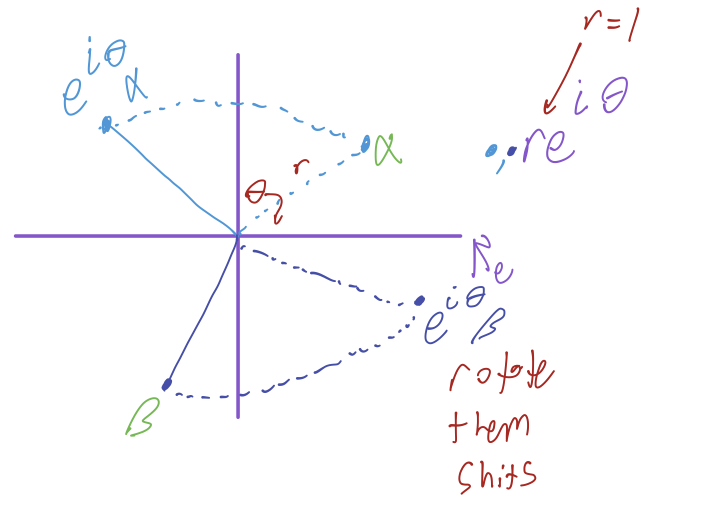
\includegraphics[width=.6\linewidth]{rotation1.jpeg}
  \centering
  \caption{Rotate}
  \label{fig:rotate1}
\end{figure}
In figure \ref{fig:rotate1}, we can see that $\ket{\psi_1}=\alpha\ket{0}+\beta\ket{1}$, and $\ket{\psi_2}=e^{i\theta}\alpha\ket{0}+e^{i\theta}\beta\ket{1}$. Basically, instead of using vectors, we're going to use density matrices. Take $\ket{\psi}\in C^2 \longrightarrow \rho_\psi =\ket{\psi}\bra{\psi}$.
\begin{center}
$\rho_\psi=\ket{\psi_1}\bra{\psi_2}=(\alpha\ket{0}+\beta\ket{1}\cdot(\alpha^*\bra{0}+\beta^*\bra{1}$\\
$=\abs{\alpha}^2\ket{0}\bra{0}+\alpha\beta^*\ket{0}\bra{1}+\beta\alpha^*\ket{1}\bra{0}+\abs{\beta}^2\ket{1}\bra{1}$\\
$\bmat{\abs{\alpha}^2 & \alpha\beta^* \\ \beta\alpha^2 & \abs{\beta}^*} =\rho\ket{\psi_1}$
\end{center}
Note that $\text{det}=0$, $\text{rank}=1$, IE the state is not entangled and not invertable. This matrix encodes all information that we can get out of $\ket{\psi}$. That is, repeated experiments can give us more information about the system, but we can't gather much more out of $\ket{\psi}$.
\begin{center}
$\longrightarrow e^{i\theta}\alpha(e^{i\theta}\alpha)^*=e^{i\theta}\alpha e^{-i\theta}\alpha^*=\alpha\alpha^*=\abs{\alpha}^*$\\
$\longrightarrow \rho_{\ket{\psi_2}}=\rho\ket{\psi_2}$ \\
$=\bmat{\abs{\alpha}^2 & \alpha\beta^* \\ \alpha^*\beta & \abs{\beta}^2}$
\end{center}
\end{example}
OK great now we're motivated about density matrices. Here's a more specific example:
\begin{example}
Given $\ket{\psi}=\frac{1}{\sqrt{2}}(\ket{0}-\ket{1})$, find the density matrix $\rho_\psi$ with respect to $\lb\ket{0},\ket{1}\rb$.
\begin{center}
$\bmat{-\frac{1}{2} & \frac{1}{2} \\ -\frac{1}{2} & \frac{1}{2}}$ \\
$\rho_\psi=\ket{\psi}\bra{\psi}=\bmat{\frac{1}{\sqrt{2}} \\ -\frac{1}{\sqrt{2}}}\bmat{\frac{1}{2} & -\frac{1}{2}}=\bmat{-\frac{1}{2} & \frac{1}{2} \\ \frac{1}{2} \\ -\frac{1}{2}}$
\end{center}
\end{example}
Here are some observations: \\
If  $\ket{\psi}\in C^n$ is a state,
\begin{itemize}
\item $\rho_\psi\in M_n(\C)$
\item $\rho_\psi$ has trace 1
\item $\rho_\psi$ is Hermitian (IE $\rho_\psi^\dagger=\rho_\psi$). \\ In fact, $\rho_\psi$ is also positive semi-definite (IE non-negative eigenvalues).
\end{itemize}
To formalize these observations, here are some definitions:
\begin{definition}
The \textbf{trace} of an $n\times n$ matrix is the \textit{sum} of its diagonal entries.
\end{definition}
\begin{definition}
A \textbf{density matrix} $\rho\in M_n$ is a Hermitian, positive-semidefinite matrix such that $\text{tr}(\rho)=1$
\end{definition}
Density matrices can be written with set-builder notation as follows:
\begin{center}
$\lb P(\ket{\psi}) \mid \ket{\psi} \text{ states }\in\C^n \rb$
$=\lb \ket{\psi}\bra{\psi} \mid \ket{\psi} \in\C^n \text{ states} \rb$
\end{center}
Note that this is not actually a vector space. These sets are also called 'pure states' where there is no 'noise' in the system. We're actually particularly interested in looking at unit density matrices. We can write the linear combinations with set builder notation as:
\begin{center}
$\lb \sum^{m}_{i=1} \rho_i \ket{\psi_i}\bra{\psi_i} \mid \sum^{m}_{i=1} \rho_i=1, \rho_i>0 \rb$
\end{center}
\begin{remark}
Sometimes, states will be unit vectors. Other times, they're just the sums of pure states, IE they're the sums of rank $1$ projection matrices.
\end{remark}
\begin{figure}[h]
  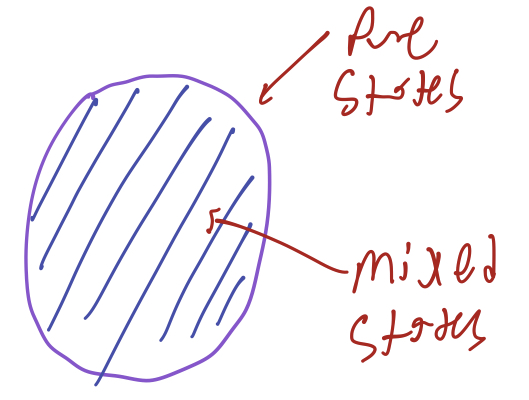
\includegraphics[width=.5\linewidth]{pure_mixed.jpeg}
  \centering
  \caption{Illustration of pure vs. mixed states}
  \label{fig:puremixed1}
\end{figure}
This set contains all complex combinations of pure states, illustrated in Figure \ref{fig:puremixed1}. This is essentially creating a weighted position average of some state $\ket{\psi}$.

%%%%%%%%%%%%%%%%%%%%%%%%%%%%%%%%%%%%%%%%%%%%%%%%%%%%%%%%%%
%%% Revisit Axiom 1 %%%
%%%%%%%%%%%%%%%%%%%%%%%%%%%%%%%%%%%%%%%%%%%%%%%%%%%%%%%%%%

\subsection{Revisit Axiom 1}
To complete computations using density matrices, it's useful to revisit Quantum Mechanics Axiom 1 discussed in section \ref{section:qma11}.
\begin{remark}
A physical state of a system, whose Hilbert space $H$ is completely determined by its associated \textit{density matrix} (IE $\text{tr}(\rho)=1\longrightarrow\text{unit condition}$) which we can think of as a map; IE $\rho:H\longrightarrow H$
\end{remark}

\begin{example}
Show that a mixed state $\rho=\sum^n_{i=1}\rho_i\ket{\psi_i}\bra{\psi_i}$ satisfies $\text{tr}(\rho)=1$. With our framework, Axiom 1 still holes.\\
First, pick a basis for $H$ (Hilbert space) Then, fix an orthonormal basis $\setofkets{e}$ for $H$. Recall that $(\rho)_{ij}$ has a "special inner product" $=\bra{e_i}\rho\ket{e_i}$ (the $\text{i}^{\text{th}}$ column of $e$. Basically, we want to isolate a specific entry of the matrix. So, 
\begin{center}
$\text{tr}(\rho)=\sum^n_{i=1}\bra{e_i}\rho\ket{e_i}=\sum^n_{i=1}\bra{e_i}\sum^n_{j=1}P_j\ket{\psi_j}\bra{\psi_j}\ket{e_j}$\\
$=\text{"evenly distributing"}$\\
$=\sum^n_{j=1}P_j\sum^n_{j=1}\inp{e_i}{\psi_i}\inp{\psi_j}{e_i}$
\end{center}
So,
\begin{center}
$\text{tr}(\rho)=\sum^n_{j=1}p_j\sum^n_{i=1}\inp{\psi_j}{e_i}\inp{e_i}{\psi_j}$\\
$=\sum^n_{j=1}P_j\bra{\psi_j}\sum^n_{i=1}\ket{e_i}\inp{e_i}{\psi_j}$\\
$=\sum^n_{j=1}P_j\inp{\psi_j}{\psi_j}=1$
\end{center}
\end{example}
OK now, here's a crazy fact: $\text{tr}(AB)=\text{tr}(BA)$, even though in general, $AB\neq BA$. This is important because the trace allows us to consider a matrix as a Hilbert space. IE, 
\begin{center}
$\text{tr}((FA)F^\dagger)=\text{tr}(F_\dagger(FA))=text{tr}(IA)=text{tr}(A)$
\end{center}

%%%%%%%%%%%%%%%%%%%%%%%%%%%%%%%%%%%%%%%%%%%%%%%%%%%%%%%%%%
%%% Revisit Axiom 2 %%%
%%%%%%%%%%%%%%%%%%%%%%%%%%%%%%%%%%%%%%%%%%%%%%%%%%%%%%%%%%

\subsection{Revisit Axiom 2}
Now, let's revisit Axiom 2 from section \ref{section:qma2}. The mean value of an observable is $\left\langle A \right\rangle=\text{tr}{\rho A}$, where $\left\langle A \right\rangle$ is the probability after many measurements. Basically, we can find the probability with density matrices instead of vectors.

%%%%%%%%%%%%%%%%%%%%%%%%%%%%%%%%%%%%%%%%%%%%%%%%%%%%%%%%%%
%%% Revisit Axiom 3 %%%
%%%%%%%%%%%%%%%%%%%%%%%%%%%%%%%%%%%%%%%%%%%%%%%%%%%%%%%%%%

\subsection{Revisit Axiom 3}
The time evolution of a density matrix is given by the Louisville-Von Neumann equation:
\begin{equation}
i\hbar \frac{d}{dt}\left[ \rho \right] = \left[ H,P \right]=H\rho-\rho H
\end{equation}



Recall that the probability of having an outcome of $\lambda$, an eigenvalue for an observable Hermitian $A$, given that the system is in state $\ket{\psi}$ is
\begin{center}
$\abs{\inp{\lambda}{\psi}}^2$
\end{center}

\begin{example}
Recall that mixed density matrices are convex combinations of pure states.
\begin{center}
$\ket{\psi}=\ket{0}=\bmat{1 \\ 0}\longrightarrow\rho=\ket{\psi}\bra{\psi}=\bmat{1 & 0 \\ 0 & 0} \text{ }50\%$\\
$\ket{\phi_1}=\ket{1}=\bmat{0 \\ 1}\longrightarrow\rho_1=\ket{1}\bra{1}=\bmat{0 & 0 \\ 0 & 1}\text{ }25\%$\\
$\ket{\phi_2}=\frac{1}{\sqrt{2}}\bmat{1 \\ -1}\longrightarrow\rho_2=\ket{phi_2}\bra{phi_2}=\frac{1}{2}\bmat{1 & -1 \\ -1 & 1} \text{ } 25\%$
\end{center}
\end{example}
In the density matrix picture, $\ket{\psi}$ is replaced by $\rho=\sum_iP_i\ket{\psi_i}\bra{\psi_i}$. The probability of outcome $\lambda$ upon measuring an observable $A$, given state $\rho$ is:
\begin{enumerate}
\item $\bra{\lambda}\rho\ket{\lambda}=\sum_iP_i\inp{\lambda}{\psi_i}\inp{\psi_i}{\lambda}$
\item $\sum_iP_i\abs{{\lambda}{\psi_i}}$ (IE weighting the state by a probability
\item $\text{tr}(\ket{\lambda}\bra{\lambda}\rho)$
\end{enumerate}
OK but what about bipartite states with density matrices? Bad news.. tensors of pure states (density matrices). Recall:\\
\begin{center}
$\ket{\psi}\in\C^n\otimes\C^n$\\
$\ket{\psi}=\sum^n_{i=1}c_i\ket{\psi}\bra{\psi}$\\
$=\ket{\psi_1}\otimes\ket{\psi_2}$
\end{center}
Basically, for vectors, separable means we can write them as a tensor. Now we're motivated to find the analog for density matrices.

\begin{definition}
Let $\rho\in M_n(\C)\otimes M_n(\C)$ be a density matrix. Recall that $\rho=\sum^n_{i=1}c_iA_{1,i}\otimes A_{2,i}$ where $A_{1,i}\in M_n(\C)$ and $A_{2,i}\in M_n(\C)$.
\end{definition}
What can we say about $\rho$?
\begin{enumerate}
\item $\rho$ is uncorrelated if $\rho_i=\rho_1\otimes\rho_2$ where $\rho_i$ is a density matrix
\item $\rho$ is "separable" if $\rho=\sum^n_{i=1}c_i\rho_{1,i}\otimes \rho_{2,i}$. Note that each $\rho_{1,i}$ and $\rho_{2,i}$ are density matrices where $\sum P_i=1$
\item If $\rho$ is not "separable", we can call $\rho$ inseparable.
\end{enumerate}
Let's see an example to tie this together.
\begin{example}
Given $\ket{02}\in\C^2\otimes\C^3$, or $\bmat{1 \\ 0}\otimes\bmat{0 \\ 0 \\ 1}=\bmat{0 \\ 0 \\ 1 \\ 0 \\ 0 \\ 0}$, consider the following:
\begin{center}
$\rho=\ket{02}\bra{02}=\bmat{0 \\ 0 \\ 1 \\ 0 \\ 0 \\ 0}\bmat{0 & 0 & 1 & 0 & 0 & 0}$
$=\bmat{
0 & 0 & 0 & 0 & 0 & 0 \\
0 & 0 & 0 & 0 & 0 & 0 \\
0 & 0 & 1 & 0 & 0 & 0 \\
0 & 0 & 0 & 0 & 0 & 0 \\
0 & 0 & 0 & 0 & 0 & 0 \\
0 & 0 & 0 & 0 & 0 & 0 \\
0 & 0 & 0 & 0 & 0 & 0
}$
\end{center}
Is this separable? Our best case scenario is $\rho=\rho_1\otimes\rho_2\in M_2\otimes M_3$. In other words, we need to find the matrices that make this possible. In this case it's pretty easy:
\begin{center}
$\bmat{
1 & 0 \\
0 & 0
}\otimes\bmat{
0 & 0 & 0 \\
0 & 0 & 0 \\
0 & 0 & 1
}=\rho=\bmat{
0 & 0 & 0 & 0 & 0 & 0 \\
0 & 0 & 0 & 0 & 0 & 0 \\
0 & 0 & 1 & 0 & 0 & 0 \\
0 & 0 & 0 & 0 & 0 & 0 \\
0 & 0 & 0 & 0 & 0 & 0 \\
0 & 0 & 0 & 0 & 0 & 0 \\
0 & 0 & 0 & 0 & 0 & 0
}=E_{33}\in M_6$
\end{center}
Therefore, $\rho$ is both pure AND uncorrelated.
\end{example}
\begin{definition}
Suppose $A\in M_n(\C)\otimes M_m(\C)$. The \textbf{partial trace} of $A$ over $\C^m$ is
\begin{equation}
A=\sum^n_{i=1}c_iA_{1,i}\otimes A_{2,i}
\end{equation}
\begin{equation}
A_1=\text{tr}_2(A)\sum^n_{i=1}c_iA_{1,i}\cdot\text{tr}(A_{2,i})\in M_n
\end{equation}
Basically, if we add a bunch of $M_n$ matrices, we get another $M_n$ matrix.
\begin{equation}
A_2=\text{tr}_1(A)\sum^n_{i=1}c_i\text{tr}A_{1,i}\cdot A_{2,i}\in M_n
\end{equation}
\end{definition}
Note that these don't live inside the tensor anymore..

\begin{example}
What can we say about
$\ket{\psi}=\frac{1}{\sqrt{2}}(\ket{01}\otimes\ket{10})$?\\
\begin{center}
$\rho=\ket{\psi}\bra{\psi}=\frac{1}{2}(\ket{01}+\ket{10})(\bra{01}+\bra{10})$\\
$=\frac{1}{2}(  \underbrace{\textstyle \ket{01}\bra{01}}_{\mathclap{E_{22}}}+\underbrace{\textstyle \bra{10}\ket{10}}_{\mathclap{E_{23}}}+\underbrace{\textstyle \bra{01}\ket{01}}_{\mathclap{E_{32}}}+\underbrace{\textstyle \ket{10}\bra{10}}_{\mathclap{E_{33}}})\in M_2\otimes M_2$\\
$=\frac{1}{2}\bmat{
0 & 0 & 0 & 0 \\
0 & 1 & 1 & 0 \\
0 & 1 & 1 & 0 \\
0 & 0 & 0 & 0 \\
}\in M_4$
\end{center}
OK check this out: We need to find some matrices such that
\begin{center}
$\bmat{0 & 0 \\ 0 & 1}=A_{11}B$ and $\bmat{0 & 1 \\ 0 & 0}=A_{21}B$ and ...
\end{center}
However, no such "$B$" can exist, since they all contradict each other! Therefore, these states are NOT uncorrelated.
\end{example}

%%%%%%%%%%%%%%%%%%%%%%%%%%%%%%%%%%%%%%%
%%%%%
% Quantum Information Theory (probably)
%%%%%
%%%%%%%%%%%%%%%%%%%%%%%%%%%%%%%%%%%%%%%

\section{Quantum Information Theory (probably)}

Quick highlights reel of my life as a computer scientist so far:

%%%%%%%%%%%%%%%%%%%%%%%%%%%%%%%%%%%%%%%%%%%%%%%%%%%%%%%%%%
%%% Classical framework of Information Theory  %%%
%%%%%%%%%%%%%%%%%%%%%%%%%%%%%%%%%%%%%%%%%%%%%%%%%%%%%%%%%%

\subsection{Classical framework of Information Theory }
\begin{itemize}
\item A classical (Boolean) bit is an element $x\in \lb 0,1 \rb$
\item Data is transmitted in strings of bits (IE a bit string)
\end{itemize}

\begin{example}
$0100$ is a bit string of length 4
\end{example}

\begin{example}
A bit string of length $8$ is a \textit{byte}. Also, $00100100$ in UTF-8 ASCII is the dollar sign (\$)
\end{example}

%%%%%%%%%%%%%%%%%%%%%%%%%%%%%%%%%%%%%%%%%%%%%%%%%%%%%%%%%%
%%% Qubits  %%%
%%%%%%%%%%%%%%%%%%%%%%%%%%%%%%%%%%%%%%%%%%%%%%%%%%%%%%%%%%

\subsection{Qubits}
\begin{definition}
A \textbf{qubit} is a unit vector in $\C^2$, IE
$\ket{\psi}=a\ket{0}+b\ket{1}$ such that $\abs{a}^2+\abs{b}^2=1$
\end{definition}
\begin{itemize}
\item To extract information form a qubit, we somehow have to \textit{measure} it, which results in \textit{collapse} to either $\ket{0}$ or $\ket{1}$.
\item Qutrits ($\C^3$) and qudits($\C^4$) also exist
\end{itemize}
\begin{definition}
A group/system of $n$ qubits is called a \textbf{quantum register}.
\end{definition}
Quick classical example to motivate the idea of quantum registers:
\begin{example}
$xyzw$ is a bit string of length $4$, and is completely determined by the values of $x,y,z,w$ independent of each other. Basically, there are $4$ values out of $2^4$ possibilities.
\end{example}
OK, suppose we describe a quantum register of $n$-qubits analogous to the classical framework, meaning that we can write each qubit as
\begin{center}
$a_i\ket{0}+b_1\ket{1}$ for $i=1,...,n$\\
$(a_1\ket{0}+b_1\ket{1})\otimes (a_2\ket{0}+b_2\ket{1})\otimes ...\otimes (a_n\ket{0}+b_n\ket{1})$
\end{center}
This is sick, but not every state in a tensor product has this form, which means it's entangled. So, the state of the system
\begin{center}
$\ket{\psi}=\sum_{i_k=0}a_i\cdot i_2 \cdot i_n \ket{i_1}\otimes \ket{i_2}\otimes ... \otimes \ket{i_n}\in\C^{2^n}$ (holy shit)
\end{center}
is a linear combination of basis vectors.

\begin{example}
Suppose we have two qubits (unit vectors in $\C^2\otimes\C^2$). 
The set 
\begin{center}
$\lb\ket{\Phi^{+}}=\frac{1}{\sqrt{2}}(\ket{00}+\ket{11}),\ket{\Phi^{-}}=\frac{1}{\sqrt{2}}(\ket{00}-\ket{11}),\ket{\Psi^{+}}=\frac{1}{\sqrt{2}}(\ket{01}+\ket{10}),\ket{\Psi^{-}}=\frac{1}{\sqrt{2}}(\ket{01}-\ket{10})\rb$
\end{center}
is called the Bell Basis, and is an orthonormal basis for $\C^2\otimes\C^2$. Each Bell State is entangled!
\end{example}
Back to classical land to motivate transmission of data with qubits:
\begin{example}\label{ex:crc}
(Classical Repition Code) Suppose a user wants to send the message $1011$ over some communication channel. Check it out: 
\begin{center}
	$1011\longrightarrow 1001$ IE data loss
\end{center}
We can encode (super elementary) redundancy using $4$ blocks of $4$-bits.
\begin{center}
	$1011\longrightarrow \underbrace{\textstyle 1111000011111111}_{\text{send this}}$
\end{center}
What if we receive $1111010011010111$? By simple majority, we can see that we encountered some sort of data loss in this transmission.
\end{example}
OK siiick now how can we do this with Qubits? First, here are some operations:
\begin{itemize}
	\item Measurement, IE collapse $\longrightarrow$ not ideal
	\item Unitary transformation $\longrightarrow$ spin matrices (IE quantum gates)
\end{itemize}
Here is our first QIT theorem of the semester that illustrates whether example \ref{ex:crc} is possible in quantum land.
\begin{theorem}
	(Non-Cloning Theorem)\\
	An unknown quantum system cannot be cloned by unitary transformations.
\end{theorem}
Basically, if we want to encode things with QIT, we need to develop new tools. IE, there is no such unitary operator $u$ on $H\otimes H$ for all normalized states $\ket{\psi},\ket{e}\in H$ such that
$u(\ket{\psi_e})=\ket{\psi\psi}$

%%%%%%%%%%%%%%%%%%%%%%%%%%%%%%%%%%%%%%%%%%%%%%%%%%%%%%%%%%
%%% Measuring Qubits  %%%
%%%%%%%%%%%%%%%%%%%%%%%%%%%%%%%%%%%%%%%%%%%%%%%%%%%%%%%%%%

\subsection{Measuring Qubits}
Measurement is basically enacting some operation on a system to output a classical bit. This operation is called collapse. To illustrate this operation, we consider a single qubit system in state $\ket{x}=a\ket{0}+b\ket{1}$. The goal is to find the probability that the state in question is $\ket{0}$ ($+1$ outcome) or $\ket{1}$ ($-1$ outcome) upon measurement. Basically, we want to use the spectral projections associated with $\sigma_z=\bmat{1 & 0 \\ 0 & -1}$.
\begin{center}
$=\underbrace{1}_{\lambda_1}\underbrace{\ket{0}\bra{0}}_{M_0}+\underbrace{(-1)}_{\lambda_2}\underbrace{\proj{1}{1}}_{M_1}$\\
$P(0)=a^2=\bra{x}M_0\ket{x}$\\
$P(1)=b^2=\bra{x}M_1\ket{x}$
\end{center}
With this motivation, let's complete an example in a bi-partite system.
\begin{example}
Let $\ket{\psi}$ be a state in a $2$-qubit system.
\begin{center}
$\ket{\psi}=a\ket{00}+b\ket{01}+c\ket{10}+d\ket{11}$
\end{center} 
Suppose we want to find the probability that the first qubit is $\ket{0}$ or $\ket{1}$ after measurement of $\ket{\psi}$. Basically, we want to consider the observable associated to the Hermitian matrix $A=\sigma_z\otimes I_2$. This means that we should consider the projection operators
\begin{center}
$M_0=\proj{0}{0}\otimes I_2$\\
$M_1=\proj{1}{1}\otimes I_2$
\end{center}
We tensor by $I_2$ to leave the second qubit alone, and only operate on the first one in the system.
\begin{center}
$\ket{\psi}=\ket{0}\otimes (a\ket{0}+b\ket{1})+\ket{1}\otimes (c\ket{0}+d\ket{1})$\\
$=u\ket{0}\otimes (\frac{a}{u}\ket{0}+\frac{b}{u}\ket{1})+\ket{v}\otimes (\frac{c}{v}\ket{0}+\frac{d}{v}\ket{1})$
\end{center}
where
\begin{center}
$u=\sqrt{\abs{a}^2+\abs{b}^2}$
\end{center}
and
\begin{center}
$v=\sqrt{\abs{c}^2+\abs{d}^2}$
\end{center}
OK, now, let's do our projections with these new $M_0$ and $M_1$.
\begin{center}
$P(0)=\bra{\psi}M_0\ket{\psi}=u^2$\\
$P(1)=\bra{\psi}M_1\ket{\psi}=v^2$
\end{center}
More specifically, we're collapsing onto $\ket{0}\otimes (a\ket{0}+b\ket{1})$ and $\ket{1}\otimes (c\ket{0}+d\ket{0})$
\end{example}
\begin{example}
Consider $\ket{\Phi^+}=\frac{1}{\sqrt{2}}(\ket{00}+\ket{11})$. We want to measure the system to determine vertical/horizontal polarization.
\begin{center}
($\sigma_z$ spectral projections)
$M_0=\ket{0}\bra{0}=\bmat{1 & 0 \\ 0 & 0}$\\
$M_1=\ket{1}\bra{1}=\bmat{0 & 0 \\ 0 & 1}$
\end{center}
Basically, on the first qubit, we have $M_0\otimes I$ and $M_1\otimes I$.
\begin{center}
$\ket{\Phi^+}=\frac{1}{\sqrt{2}}\ket{0}\otimes\ket{0}+0\ket{0}\otimes\ket{1}+0\ket{1}\otimes\ket{0}+\frac{1}{\sqrt{2}}\ket{1}\otimes\ket{1}$\\
$=\frac{1}{\sqrt{2}}\ket{0}\otimes(\ket{0}+0\ket{1})+\frac{1}{\sqrt{2}}\ket{1}\otimes(0\ket{0}+\ket{1})$
($M_0\otimes I\ket{\Phi^+}$)\\
$=\frac{1}{\sqrt{2}}\ket{0}\inp{0}{0}\otimes (\ket{0}\otimes 0\ket{1})+0$\\
$=\frac{1}{\sqrt{2}}\ket{0}\otimes (\ket{0}+0)=\frac{1}{\sqrt{2}}\ket{0}\otimes \ket{0}$\\
$\bra{\Phi^+}M_0\otimes I\ket{\Phi^+}$\\
$=\frac{1}{2}(1+0)=\frac{1}{2}$
\end{center}
Therefore, the actual probability that the particle will be horizontal in the first qubit is $\frac{1}{2}$.
\end{example}
Recall that measurement causes collapse. So what now? Well, we found that $\ket{\Phi^+}$ collapses to $\frac{1}{\sqrt{2}}\ket{0}\otimes (\ket{0}+0\ket{1})$, but note that the measurement also affected the second qubit.

%%%%%%%%%%%%%%%%%%%%%%%%%%%%%%%%%%%%%%%%%%%%%%%%%%%%%%%%%%
%%% BB84 Protocol for Quantum Key Distribution (QKD)   %%%
%%%%%%%%%%%%%%%%%%%%%%%%%%%%%%%%%%%%%%%%%%%%%%%%%%%%%%%%%%

\subsection{BB84 Protocol for Quantum Key Distribution (QKD)}
A nice example of single qubit measurement is quantum key distribution. Key distribution is a cryptographic concept that pertains to the production and distribution of a key to two parties wishing to communicate securely, by means of encrypting and decryption methods. The unique benefit of quantum key distribution is that two communicating parties can detect eavesdropping of the transfer of keys due to the quantum principal that in general, measurement results in disturbance and often collapse of the system. To i
\begin{example}
Suppose Alice and Bob are using a \textit{one-time pad} encryption technique to communicate with each other. Alice wants to send the byte $00100100$ to Bob. They use the BB84 protocol to distribute the encryption key for communication. First, they use the bases $\beta_1$ and $\beta_2$ to prepare and measure $4N=32$ photons.
\begin{center}
$\beta_1=\lb\substack{0\mapsto\ket{0}\\1\mapsto\ket{1}}\rb$ and $\beta_2=\lb\substack{0\mapsto\ket{\nearrow}=\frac{1}{\sqrt{2}}(\ket{0}+\ket{1})\\1\mapsto\ket{\searrow}=\frac{1}{\sqrt{2}}(\ket{0}-\ket{1})}\rb$
\end{center}
Then, Alice sends Bob these $4N=32$ photons, each prepared with one of the two bases $\beta_1$ and $\beta_2$ at random.
\begin{center}
\begin{table}[h]
\centering
\begin{tabular}{|l|l|l|l|l|l|l|l|l|l|l|l|l|l|l|l|l|l}
\hline
\textbf{Alice sends} & 0 & 1 & 0 & 0 & 1 & 1 & 0 & 1 & 0 & 0 & 1 & 0 & 0 & 0 & 1 & 0 & ... \\ \hline
\textbf{Alice's basis} & $\beta_1$ & $\beta_2$ & $\beta_1$ & $\beta_2$ & $\beta_2$ & $\beta_1$ & $\beta_2$ & $\beta_1$ & $\beta_2$ & $\beta_2$ & $\beta_1$ & $\beta_1$ & $\beta_1$ & $\beta_1$ & $\beta_2$ & $\beta_1$ & ... \\ \hline
\end{tabular}
\end{table}
\end{center}
Now, Bob measures each received photons with respect to one of each of the two bases at random.
\begin{center}
\begin{table}[h]
\centering
\begin{tabular}{|l|l|l|l|l|l|l|l|l|l|l|l|l|l|l|l|l|l}
\hline
\textbf{Alice sends} & 0 & 1 & 0 & 0 & 1 & 1 & 0 & 1 & 0 & 0 & 1 & 0 & 0 & 0 & 1 & 0 & ... \\ \hline
\textbf{Alice's basis} & $\beta_1$ & $\beta_2$ & $\beta_1$ & $\beta_2$ & $\beta_2$ & $\beta_1$ & $\beta_2$ & $\beta_1$ & $\beta_2$ & $\beta_2$ & $\beta_1$ & $\beta_1$ & $\beta_1$ & $\beta_1$ & $\beta_2$ & $\beta_1$ & ... \\ \hline
\textbf{Bob's basis} & $\beta_1$ & $\beta_2$ & $\beta_2$ & $\beta_1$ & $\beta_2$ & $\beta_2$ & $\beta_1$ & $\beta_2$ & $\beta_1$ & $\beta_2$ & $\beta_1$ & $\beta_1$ & $\beta_1$ & $\beta_1$ & $\beta_2$ & $\beta_1$ & ... \\ \hline
\textbf{Bob reads} & 0 & 1 & ? & ? & 1 & ? & ? & ? & ? & 0 & ? & 0 & ? & ? & ? & ? & ... \\ \hline
\end{tabular}
\end{table}
Where $\inp{\psi}{\nearrow}\inp{\searrow}{\psi}=\frac{1}{2}\Rightarrow 50/50$ shot $\Rightarrow$ ?
\end{center}
We can see that when Bob measures the bits sent by Alice with a basis different than the one she used, he cannot get any discernible information. Next, Alice and Bob talk over a classical line and identify the photons that were prepared and measured using the same basis, or roughly $2N=16$ photons. These photons are represented by the bits with a definitive collapse, IE non '?'. The remaining roughly $2N=16$ photons that Alice will send should be prepared and measured according to this same basis. Now, Alice and Bob select $N=8$ photons among the $2N=16$ photons at random to detect any tampering on the quantum line.
\begin{center}
\begin{table}[h]
\centering
\begin{tabular}{|l|l|l|l|l|l|l|l|l|l|l|l|l|l|l|l|l|}
\hline
\textbf{Alice sends} & 0 & 1 & 1 & 0 & 0 & 1 & 0 & 0 & 1 & 0 & 0 & 0 & 1 & 1 & 1 & 0 \\ \hline
\textbf{Alice's basis} & $\beta_1$ & $\beta_2$ & $\beta_2$ & $\beta_2$ & $\beta_1$ & $\beta_1$ & $\beta_1$ & $\beta_2$ & $\beta_1$ & $\beta_1$ & $\beta_1$ & $\beta_2$ & $\beta_1$ & $\beta_2$ & $\beta_2$ & $\beta_2$ \\ \hline
\textbf{Bob's basis} & $\beta_1$ & $\beta_2$ & $\beta_2$ & $\beta_2$ & $\beta_1$ & $\beta_1$ & $\beta_1$ & $\beta_2$ & $\beta_1$ & $\beta_1$ & $\beta_1$ & $\beta_2$ & $\beta_1$ & $\beta_2$ & $\beta_2$ & $\beta_2$ \\ \hline
\textbf{Bob reads} & 0 & 1 & 1 & 0 & 0 & 1 & 0 & 0 & 1 & 0 & 0 & 0 & 1 & 1 & 1 & 0 \\ \hline
\end{tabular}
\end{table}
\end{center}
If Eve were listening, they would have intercepted and measured the quantum photons using $\beta_1$ or $\beta_2$ at random before passing the collapsed state to Bob.
\begin{center}
\begin{table}[h]
\centering
\begin{tabular}{|l|l|l|l|l|l|l|l|l|l|l|l|l|l|l|l|l|}
\hline
\textbf{Alice sends} & 0 & 1 & 1 & 0 & 0 & 1 & 0 & 0 & 1 & 0 & 0 & 0 & 1 & 1 & 1 & 0 \\ \hline
\textbf{Alice's basis} & $\beta_1$ & $\beta_2$ & $\beta_2$ & $\beta_2$ & $\beta_1$ & $\beta_1$ & $\beta_1$ & $\beta_2$ & $\beta_1$ & $\beta_1$ & $\beta_1$ & $\beta_2$ & $\beta_1$ & $\beta_2$ & $\beta_2$ & $\beta_2$ \\ \hline
\textbf{Eve's basis} & $\beta_1$ & $\beta_2$ & $\beta_1$ & $\beta_2$ & $\beta_1$ & $\beta_2$ & $\beta_1$ & $\beta_2$ & $\beta_1$ & $\beta_1$ & $\beta_2$ & $\beta_1$ & $\beta_2$ & $\beta_2$ & $\beta_1$ & $\beta_1$ \\ \hline
\textbf{Eve reads/sends} & 0 & 1 & ? & 0 & 0 & ? & 0 & 0 & 1 & 0 & ? & ? & ? & 1 & ? & ? \\ \hline
\textbf{Bob's basis} & $\beta_1$ & $\beta_2$ & $\beta_2$ & $\beta_2$ & $\beta_1$ & $\beta_1$ & $\beta_1$ & $\beta_2$ & $\beta_1$ & $\beta_1$ & $\beta_1$ & $\beta_2$ & $\beta_1$ & $\beta_2$ & $\beta_2$ & $\beta_2$ \\ \hline
\textbf{Bob reads} & 0 & 1 & ? & 0 & 0 & ? & 0 & 0 & 1 & 0 & ? & ? & ? & 1 & ? & ? \\ \hline
\end{tabular}
\end{table}
\end{center}
What this comes down to is that Alice and Bob \textit{can absolutely} detect if Eve is EaVEsdropping. This can be easily be seen because despite Alice and Bob confirming the bases on which they communicated, Bob still received inconclusive states in the form of '?'. Said differently, the bits checked in the \textit{Bob reads} column were supposed to 'line up' at this point, SO, we can assume that somebody was in the middle.
\end{example}

%%%%%%%%%%%%%%%%%%%%%
%%% Quantum Gates %%%
%%%%%%%%%%%%%%%%%%%%%

\subsection{Quantum Gates}
Quick recap: A quantum gate is
\begin{itemize}
\item A unitary matrix; IE reversible and allows us to change basis
\item How we prepare messages
\end{itemize}
Now, we'll go over some of the basic quantum logic gates, and compare them to their classical counterparts.
\begin{itemize}
\item NOT gate\\
Classically, a not gate performs the following actions:
\begin{center}
$0\mapsto 1$ and $0\mapsto 1$
\end{center}
And as a function, the NOT gate operates as $\lb0,1\rb\mapsto\lb0,1\rb$, IE it is a bijection. A quantum not gate operates similarly. IE
\begin{center}
$\ket{0}\mapsto\ket{1}$ and $\ket{1}\mapsto\ket{0}$
\end{center}
This is done using $\sigma_x$ which is most often just called 'X'
\item AND gate\\
Classically, an and gate takes two bits, and outputs a $1$ only if the two bits are the same, and is represented as a function by $\lb0,1\rb^2\mapsto\lb0,1\rb$. A quantum and gate operates similarly. IE
\begin{center}
\[ \ket{xyz}\mapsto \begin{cases} 
      x=y=1 & \ket{xy\overline{z}}\\
      else \\
       \ket{xyz}
   \end{cases}
\]
$\ket{101}\stackrel{\makebox[0pt]{\mbox{\normalfont\tiny QAND}}}{\mapsto}\ket{101}$\\
$\ket{110}\mapsto\ket{111}$
\end{center}
The quantum and gate is often called CCNOT.
\item XOR gate\\
Classically, the exclusive or gate takes two bits as input and outputs a $1$ only if the two bits are different, and is represented as a function by $\lb0,1\rb^2\mapsto\lb0,1\rb$. A quantum exclusive or gate operates slightly differently. Check it out:
\begin{center}
$\ket{00}\mapsto\ket{00}$\\
$\ket{01}\mapsto\ket{01}$\\
$\ket{10}\mapsto\ket{11}$\\
$\ket{11}\mapsto\ket{10}$
\end{center}
\end{itemize}

Another useful quantum gate that doesn't exist classically is called the Hadamard gate, which maps the basis states
\begin{center}
$\ket{0}\mapsto\frac{1}{\sqrt{2}}(\ket{0}+\ket{1})$\\
$\ket{1}\mapsto\frac{1}{\sqrt{2}}(\ket{0}-\ket{1})$
\end{center}
and is used to create an equal superposition of the two states. The Hadamard gate is represented by a matrix as $H=\frac{1}{\sqrt{2}}\bmat{1 & 1 \\ 1 & -1}$. See the exercises for examples of these; we didn't do many in class.

%%%%%%%%%%%%%%%%%%%%%%%%%%%%%%%%%%%%%%%%%
%%% Quantum Gates as Density Matrices %%%
%%%%%%%%%%%%%%%%%%%%%%%%%%%%%%%%%%%%%%%%%

\subsection{Quantum Gates as Density Matrices}
Quick motivation for the usefulness of density matrices representing quantum gates. The biggest question here is "what happens if quantum gates aren't dependable?" For example, noise in the quantum line or broken circuits could cause disturbances in the data transmitted.
\begin{example}
Imagine we want to send the bit $\ket{10}$ as $\ket{11}$ by applying CNOT. Maybe $80\%$ of the time $\ket{11}$ is sent. Fantastic! But, $15\%$ of the time, $(H\otimes I)\ket{10}$ is sent, and $5\%$ of the time $(H\otimes H)CNOT(H\otimes H)$ is sent. IE, the vector received is
\begin{center}
$0.80\text{CNOT}\ket{10}+0.15(H\otimes I)\ket{10}+0.05\text{CNOT}'\ket{10}$
\end{center}
Low key gross.. But what if we could just send a density matrix??
\end{example}
Well, first, we need to answer the question of how does the density matrix $\rho$ evolve under a quantum unitary gate $U$? Vector evolution allows us to apply $U$ as $\ket{\psi}\mapsto U\ket{\psi}$.
\begin{theorem}
If $\rho$ is a pure state density matrix $\rho=\ket{\psi}\bra{\psi}$ for some $\ket{\psi}\in\C^n$,
\begin{center}
$\rho=\ket{\psi}\bra{\psi}\mapsto (u\ket{\psi})(u\ket{\psi})^\dagger=U\ket{\psi}\bra{\psi}U^\dagger=U\rho U^\dagger$
\end{center}
\end{theorem}
We kind of ran out of time here... But there are some cool examples of this application in the exercises.

%%%%%%%%%%%%%%%%%%%%%%%%%%%%%%%%%%%%%%%%%%%%%%%%%%%
%%% Light speed overview of Quantum Decoherence %%%
%%%%%%%%%%%%%%%%%%%%%%%%%%%%%%%%%%%%%%%%%%%%%%%%%%%

\subsection{Light speed overview of Quantum Decoherence}
Let's talk about a possibly multipartite Hilbert system $H_S\otimes H_{\epsilon}$, which is our hypothetical environment's quantum system. Suppose we only want to measure information about $\ket{\psi}\in H_S$, but when we measure, our environment has state $\ket{\phi}\in H_{\epsilon}$. Basically, we're actually measuring $\ket{\psi}\otimes\ket{\phi}\in H_S\otimes H_{\epsilon}$, which is represented by the density matrix $(\ket{\psi}\otimes\ket{\phi})(\ket{\psi}\otimes\ket{\phi})^\dagger$. So, in a perfectly isolated quantum system, we would measure $\rho_S$ as it's actually represented supported by our axioms. But, if noise is introduced to the system during an action like measurement, coherence in the system is lost. Basically, quantum decoherence makes our density matrix $\bmat{\abs{\alpha}^2 & \alpha\beta^* \\ \beta\alpha^2 & \abs{\beta}^*}$ slowly approach $\bmat{\sim0 & \alpha\beta^* \\ \beta\alpha^2 & \sim0}$. Eventually, it becomes something that is no longer a density matrix and no longer useful to us...\\\\\\\\ok bye

%%!!!!!!!!!!!!!!!!!!!!!!!!!!!!!!!!!!!!!!!!!!!!!!!!!!!!!!!!!!!!!!!!!!!!!!!!!!!!
%%!!!!!!!!!!!!!!!!!!!!!!!!!!!!!!!!!!!!!!!!!!!!!!!!!!!!!!!!!!!!!!!!!!!!!!!!!!!!
%%!!!!!!!!!!!!!!!!!!!!!!!!!!!!!!!!!!!!!!!!!!!!!!!!!!!!!!!!!!!!!!!!!!!!!!!!!!!!
% end of document
%%!!!!!!!!!!!!!!!!!!!!!!!!!!!!!!!!!!!!!!!!!!!!!!!!!!!!!!!!!!!!!!!!!!!!!!!!!!!!
%%!!!!!!!!!!!!!!!!!!!!!!!!!!!!!!!!!!!!!!!!!!!!!!!!!!!!!!!!!!!!!!!!!!!!!!!!!!!!
%%!!!!!!!!!!!!!!!!!!!!!!!!!!!!!!!!!!!!!!!!!!!!!!!!!!!!!!!!!!!!!!!!!!!!!!!!!!!!
\end{document}